\documentclass[a4paper,11pt,fleqn]{article}

\usepackage[left=1cm,right=0.5cm,top=0.5cm,bottom=2cm]{geometry}

\usepackage{bfcours}
\usepackage{bfcours-fonts}
%\usepackage{bfcours-fonts-dys}

\def\rdifficulty{1}
\setrdexo{%left skip=1cm,
display exotitle,
exo header = tcolorbox,
%display tags,
skin = bouyachakka,
lower ={box=crep},
display score,
display level,
save lower,
score=\points,
level=\rdifficulty,
overlay={\node[inner sep=0pt,
anchor=west,rotate=90, yshift=0.3cm]%,xshift=-3em], yshift=0.45cm
at (frame.south west) {\thetags[0]} ;}
]%obligatoire
}
\setrdcrep{seyes, correction=true, correction color=monrose, correction font = \large\bfseries}

\newcommand{\tikzinclude}[1]{%
    \stepcounter{tikzfigcounter}%
    \csname tikzfig#1\endcsname
}

\newcommand{\tikzfiggGnt}{
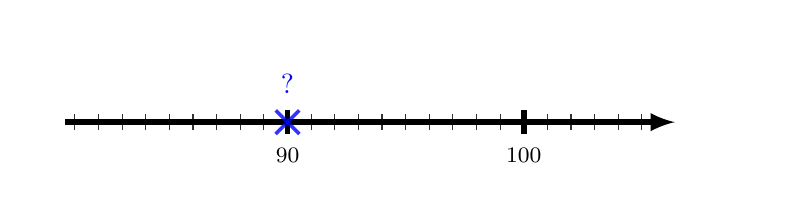
\begin{tikzpicture}[baseline,scale = 0.6]
	
		\tikzset{
		  point/.style={
			thick,
			draw,
			cross out,
			inner sep=0pt,
			minimum width=5pt,
			minimum height=5pt,
		  },
		}
		\clip (-1,-1) rectangle (15,2);
			\draw[color ={black},line width = 2,>=latex,->] (-0.2,0)--(12.7,0);
		\draw[color ={black},opacity = 0.8] (0,-0.17)--(0,0.17);
		\draw[color ={black},opacity = 0.8] (0.5,-0.17)--(0.5,0.17);
		\draw[color ={black},opacity = 0.8] (1,-0.17)--(1,0.17);
		\draw[color ={black},opacity = 0.8] (1.5,-0.17)--(1.5,0.17);
		\draw[color ={black},opacity = 0.8] (2,-0.17)--(2,0.17);
		\draw[color ={black},opacity = 0.8] (2.5,-0.17)--(2.5,0.17);
		\draw[color ={black},opacity = 0.8] (3,-0.17)--(3,0.17);
		\draw[color ={black},opacity = 0.8] (3.5,-0.17)--(3.5,0.17);
		\draw[color ={black},opacity = 0.8] (4,-0.17)--(4,0.17);
		\draw[color ={black},line width = 2] (4.5,-0.25)--(4.5,0.25);
		\draw[color ={black},opacity = 0.8] (5,-0.17)--(5,0.17);
		\draw[color ={black},opacity = 0.8] (5.5,-0.17)--(5.5,0.17);
		\draw[color ={black},opacity = 0.8] (6,-0.17)--(6,0.17);
		\draw[color ={black},opacity = 0.8] (6.5,-0.17)--(6.5,0.17);
		\draw[color ={black},opacity = 0.8] (7,-0.17)--(7,0.17);
		\draw[color ={black},opacity = 0.8] (7.5,-0.17)--(7.5,0.17);
		\draw[color ={black},opacity = 0.8] (8,-0.17)--(8,0.17);
		\draw[color ={black},opacity = 0.8] (8.5,-0.17)--(8.5,0.17);
		\draw[color ={black},opacity = 0.8] (9,-0.17)--(9,0.17);
		\draw[color ={black},line width = 2] (9.5,-0.25)--(9.5,0.25);
		\draw[color ={black},opacity = 0.8] (10,-0.17)--(10,0.17);
		\draw[color ={black},opacity = 0.8] (10.5,-0.17)--(10.5,0.17);
		\draw[color ={black},opacity = 0.8] (11,-0.17)--(11,0.17);
		\draw[color ={black},opacity = 0.8] (11.5,-0.17)--(11.5,0.17);
		\draw[color ={black},opacity = 0.8] (12,-0.17)--(12,0.17);
		\draw (4.5,-0.7) node[anchor = center] {\footnotesize \color{black}{$90$}};
		\draw (9.5,-0.7) node[anchor = center] {\footnotesize \color{black}{$100$}};
		\draw[color ={blue},line width = 1.25,opacity = 0.8] (4.25,0.25)--(4.75,-0.25);\draw[color ={blue},line width = 1.25,opacity = 0.8] (4.25,-0.25)--(4.75,0.25);
		\draw (4.5,0.8) node[anchor = center, rotate=0] {\normalsize \color{blue}{$?$}};
	
	\end{tikzpicture}
}

\newcommand{\tikzfigUfpC}{
\begin{tikzpicture}[baseline,scale = 0.8]
	
		\tikzset{
		  point/.style={
			thick,
			draw,
			cross out,
			inner sep=0pt,
			minimum width=5pt,
			minimum height=5pt,
		  },
		}
		\clip (-1.5,-1) rectangle (5,4);
			\draw [color={black}] (2,-0.5) node[anchor = center,scale=1, rotate = 0] {8,5 cm};
		\draw [color={black}] (2,3.5) node[anchor = center,scale=1, rotate = 0] {8,5 cm};
		\draw [color={black}] (4.5,1.5) node[anchor = center,scale=1, rotate = 0] {?};
		\draw[color ={black}] (0,0)--(4,0);
		\draw[color ={black}] (4,0)--(4,3);
		\draw[color ={black}] (4,3)--(0,3);
		\draw[color ={black}] (0,3)--(0,0);
		\draw[color={black},line width = 0.5] (4,0)--(3.6,0)--(3.6,0.4)--(4,0.4)--cycle;
		\draw[color={black},line width = 0.5] (4,3)--(4,2.6)--(3.6,2.6)--(3.6,3)--cycle;
		\draw[color={black},line width = 0.5] (0,3)--(0.4,3)--(0.4,2.6)--(0,2.6)--cycle;
		\draw[color={black},line width = 0.5] (0,0)--(0,0.4)--(0.4,0.4)--(0.4,0)--cycle;
	
	\end{tikzpicture}
}

\newcommand{\tikzfigaETb}{
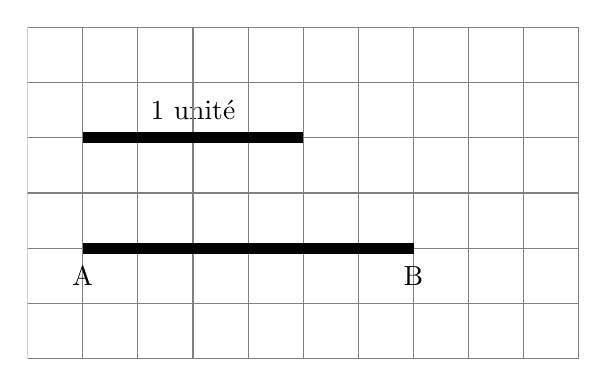
\begin{tikzpicture}[baseline,scale = 0.7]
	
		\tikzset{
		  point/.style={
			thick,
			draw,
			cross out,
			inner sep=0pt,
			minimum width=5pt,
			minimum height=5pt,
		  },
		}
		\clip (-1,-2) rectangle (9,4);
			\draw [color={black}] (2,2.5) node[anchor = center,scale=1, rotate = 0] {1 unité};
		\draw[color ={gray}] (-2,-2)--(-2,4);
		\draw[color ={gray}] (-1,-2)--(-1,4);
		\draw[color ={gray}] (0,-2)--(0,4);
		\draw[color ={gray}] (1,-2)--(1,4);
		\draw[color ={gray}] (2,-2)--(2,4);
		\draw[color ={gray}] (3,-2)--(3,4);
		\draw[color ={gray}] (4,-2)--(4,4);
		\draw[color ={gray}] (5,-2)--(5,4);
		\draw[color ={gray}] (6,-2)--(6,4);
		\draw[color ={gray}] (7,-2)--(7,4);
		\draw[color ={gray}] (8,-2)--(8,4);
		\draw[color ={gray}] (9,-2)--(9,4);
		\draw[color ={gray}] (-2,-2)--(9,-2);
		\draw[color ={gray}] (-2,-1)--(9,-1);
		\draw[color ={gray}] (-2,0)--(9,0);
		\draw[color ={gray}] (-2,1)--(9,1);
		\draw[color ={gray}] (-2,2)--(9,2);
		\draw[color ={gray}] (-2,3)--(9,3);
		\draw[color ={gray}] (-2,4)--(9,4);
		\draw[color ={black},line width = 4] (0,2)--(4,2);
		\draw[color ={black},line width = 4] (0,0)--(6,0);
		\draw [color={black}] (0,-0.5) node[anchor = center,scale=1, rotate = 0] {A};
		\draw [color={black}] (6,-0.5) node[anchor = center,scale=1, rotate = 0] {B};
	
	\end{tikzpicture}
}

\newcommand{\tikzfigeYEf}{
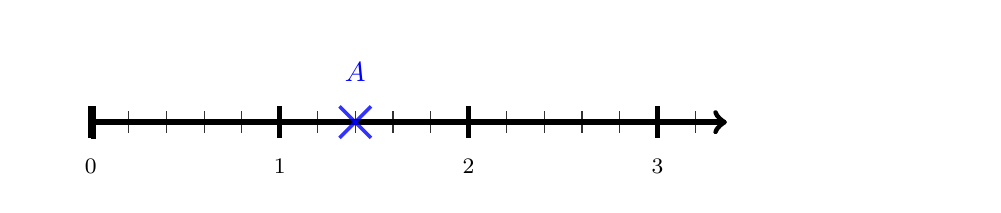
\begin{tikzpicture}[baseline,scale = 0.8]
	
		\tikzset{
		  point/.style={
			thick,
			draw,
			cross out,
			inner sep=0pt,
			minimum width=5pt,
			minimum height=5pt,
		  },
		}
		\clip (-1,-1) rectangle (14,1.5);
			\draw[color ={black},line width = 2,|->] (0,0)--(10.1,0);
		\draw[color ={black},line width = 2] (0,-0.25)--(0,0.25);
		\draw[color ={black},opacity = 0.8] (0.6,-0.17)--(0.6,0.17);
		\draw[color ={black},opacity = 0.8] (1.2,-0.17)--(1.2,0.17);
		\draw[color ={black},opacity = 0.8] (1.8,-0.17)--(1.8,0.17);
		\draw[color ={black},opacity = 0.8] (2.4,-0.17)--(2.4,0.17);
		\draw[color ={black},line width = 2] (3,-0.25)--(3,0.25);
		\draw[color ={black},opacity = 0.8] (3.6,-0.17)--(3.6,0.17);
		\draw[color ={black},opacity = 0.8] (4.2,-0.17)--(4.2,0.17);
		\draw[color ={black},opacity = 0.8] (4.8,-0.17)--(4.8,0.17);
		\draw[color ={black},opacity = 0.8] (5.4,-0.17)--(5.4,0.17);
		\draw[color ={black},line width = 2] (6,-0.25)--(6,0.25);
		\draw[color ={black},opacity = 0.8] (6.6,-0.17)--(6.6,0.17);
		\draw[color ={black},opacity = 0.8] (7.2,-0.17)--(7.2,0.17);
		\draw[color ={black},opacity = 0.8] (7.8,-0.17)--(7.8,0.17);
		\draw[color ={black},opacity = 0.8] (8.4,-0.17)--(8.4,0.17);
		\draw[color ={black},line width = 2] (9,-0.25)--(9,0.25);
		\draw[color ={black},opacity = 0.8] (9.6,-0.17)--(9.6,0.17);
		\draw (0,-0.7) node[anchor = center] {\footnotesize \color{black}{$0$}};
		\draw (3,-0.7) node[anchor = center] {\footnotesize \color{black}{$1$}};
		\draw (6,-0.7) node[anchor = center] {\footnotesize \color{black}{$2$}};
		\draw (9,-0.7) node[anchor = center] {\footnotesize \color{black}{$3$}};
		\draw[color ={blue},line width = 1.25,opacity = 0.8] (3.95,0.25)--(4.45,-0.25);\draw[color ={blue},line width = 1.25,opacity = 0.8] (3.95,-0.25)--(4.45,0.25);
		\draw (4.199999999999999,0.8) node[anchor = center, rotate=0] {\normalsize \color{blue}{$A$}};
	
	\end{tikzpicture}
}

\newcommand{\tikzfigocLB}{

\begin{tikzpicture}[baseline,scale = 0.3]

    \tikzset{
      point/.style={
        thick,
        draw,
        cross out,
        inner sep=0pt,
        minimum width=5pt,
        minimum height=5pt,
      },
    }
    \clip (-0.7,-2.7) rectangle (7.7,0.7);
    	
	 \filldraw[color={black},fill={black}] (0,0) circle (0.2);
	
	 \filldraw[color={black},fill={black}] (1,0) circle (0.2);
	
	 \filldraw[color={black},fill={black}] (2,0) circle (0.2);
	
	 \filldraw[color={black},fill={black}] (3,0) circle (0.2);
	
	 \filldraw[color={black},fill={black}] (4,0) circle (0.2);
	
	 \filldraw[color={black},fill={black}] (5,0) circle (0.2);
	
	 \filldraw[color={black},fill={black}] (6,0) circle (0.2);
	
	 \filldraw[color={black},fill={black}] (7,0) circle (0.2);
	
	 \filldraw[color={black},fill={black}] (0,-1) circle (0.2);
	
	 \filldraw[color={black},fill={black}] (1,-1) circle (0.2);
	
	 \filldraw[color={black},fill={black}] (2,-1) circle (0.2);
	
	 \filldraw[color={black},fill={black}] (3,-1) circle (0.2);
	
	 \filldraw[color={black},fill={black}] (4,-1) circle (0.2);
	
	 \filldraw[color={black},fill={black}] (5,-1) circle (0.2);
	
	 \filldraw[color={black},fill={black}] (6,-1) circle (0.2);
	
	 \filldraw[color={black},fill={black}] (7,-1) circle (0.2);
	
	 \filldraw[color={black},fill={black}] (0,-2) circle (0.2);
	
	 \filldraw[color={black},fill={black}] (1,-2) circle (0.2);
	
	 \filldraw[color={black},fill={black}] (2,-2) circle (0.2);
	
	 \filldraw[color={black},fill={black}] (3,-2) circle (0.2);
	
	 \filldraw[color={black},fill={black}] (4,-2) circle (0.2);
	
	 \filldraw[color={black},fill={black}] (5,-2) circle (0.2);
	
	 \filldraw[color={black},fill={black}] (6,-2) circle (0.2);
	
	 \filldraw[color={black},fill={black}] (7,-2) circle (0.2);

\end{tikzpicture}
}

\newcommand{\tikzfigfUFI}{
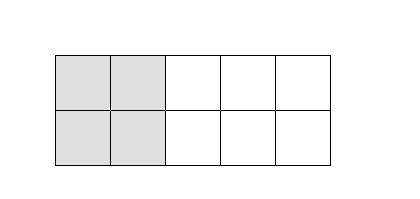
\begin{tikzpicture}[baseline,scale = 0.7]

    \tikzset{
      point/.style={
        thick,
        draw,
        cross out,
        inner sep=0pt,
        minimum width=5pt,
        minimum height=5pt,
      },
    }
    \clip (-0.5,-0.1) rectangle (6.1,2.5);
    	\draw[color={black},preaction={fill,color = {lightgray}, opacity = 0.5}] (0,0)--(2,0)--(2,2)--(0,2)--(0,2)--(0,2)--cycle;
	\draw[color ={black}] (0,0)--(0,2);
	\draw[color ={black}] (1,0)--(1,2);
	\draw[color ={black}] (2,0)--(2,2);
	\draw[color ={black}] (3,0)--(3,2);
	\draw[color ={black}] (4,0)--(4,2);
	\draw[color ={black}] (5,0)--(5,2);
	\draw[color ={black}] (0,0)--(5,0);
	\draw[color ={black}] (0,1)--(5,1);
	\draw[color ={black}] (0,2)--(5,2);

\end{tikzpicture}
}

\newcommand{\tikzfiggJBH}{
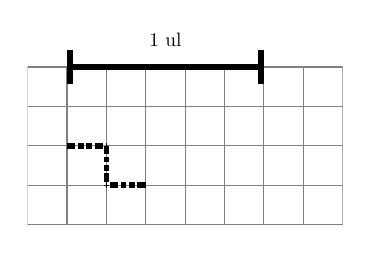
\begin{tikzpicture}[baseline,scale = 0.5]

    \tikzset{
      point/.style={
        thick,
        draw,
        cross out,
        inner sep=0pt,
        minimum width=5pt,
        minimum height=5pt,
      },
    }
    \clip (-1,-0.2) rectangle (7,5);
    	\draw [color={black}] (2.5,4.7) node[anchor = center,scale=0.7, rotate = 0] {1 ul};
	\draw[color ={gray}] (-2,0)--(-2,4);
	\draw[color ={gray}] (-1,0)--(-1,4);
	\draw[color ={gray}] (0,0)--(0,4);
	\draw[color ={gray}] (1,0)--(1,4);
	\draw[color ={gray}] (2,0)--(2,4);
	\draw[color ={gray}] (3,0)--(3,4);
	\draw[color ={gray}] (4,0)--(4,4);
	\draw[color ={gray}] (5,0)--(5,4);
	\draw[color ={gray}] (6,0)--(6,4);
	\draw[color ={gray}] (7,0)--(7,4);
	\draw[color ={gray}] (-2,0)--(7,0);
	\draw[color ={gray}] (-2,1)--(7,1);
	\draw[color ={gray}] (-2,2)--(7,2);
	\draw[color ={gray}] (-2,3)--(7,3);
	\draw[color ={gray}] (-2,4)--(7,4);
	\draw[color ={black},line width = 2,|-|] (0,4)--(5,4);
	\draw[color ={black},line width = 2, densely dash dot dot ] (0,2)--(1,2);
	\draw[color ={black},line width = 2, densely dash dot dot ] (1,2)--(1,1);
	\draw[color ={black},line width = 2, densely dash dot dot ] (2,1)--(1,1);

\end{tikzpicture}
}

\newcommand{\tikzfigXsHR}{
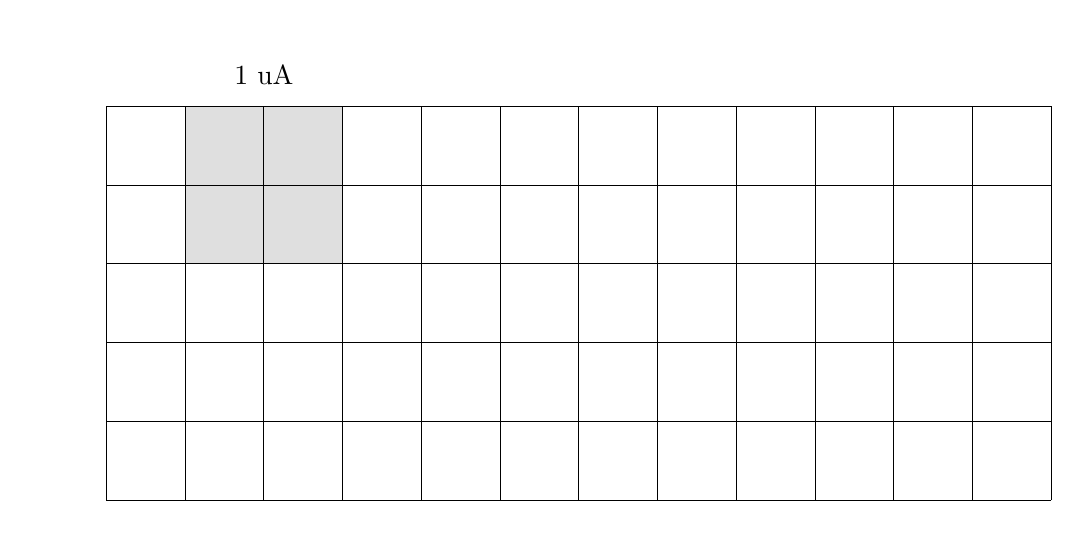
\begin{tikzpicture}[baseline]

    \tikzset{
      point/.style={
        thick,
        draw,
        cross out,
        inner sep=0pt,
        minimum width=5pt,
        minimum height=5pt,
      },
    }
    \clip (-1,-0.1) rectangle (12.1,6);
    	\draw[color={black},preaction={fill,color = {lightgray}, opacity = 0.5}] (1,5)--(3,5)--(3,3)--(1,3)--cycle;
	\draw[color ={black}] (0,0)--(0,5);
	\draw[color ={black}] (1,0)--(1,5);
	\draw[color ={black}] (2,0)--(2,5);
	\draw[color ={black}] (3,0)--(3,5);
	\draw[color ={black}] (4,0)--(4,5);
	\draw[color ={black}] (5,0)--(5,5);
	\draw[color ={black}] (6,0)--(6,5);
	\draw[color ={black}] (7,0)--(7,5);
	\draw[color ={black}] (8,0)--(8,5);
	\draw[color ={black}] (9,0)--(9,5);
	\draw[color ={black}] (10,0)--(10,5);
	\draw[color ={black}] (11,0)--(11,5);
	\draw[color ={black}] (12,0)--(12,5);
	\draw[color ={black}] (0,0)--(12,0);
	\draw[color ={black}] (0,1)--(12,1);
	\draw[color ={black}] (0,2)--(12,2);
	\draw[color ={black}] (0,3)--(12,3);
	\draw[color ={black}] (0,4)--(12,4);
	\draw[color ={black}] (0,5)--(12,5);
	\draw [color={black}] (2,5.4) node[anchor = center,scale=1, rotate = 0] {1 uA};

\end{tikzpicture}
}

\newcommand{\tikzfigSabl}{
\begin{tikzpicture}[baseline,scale = 0.7]

    \tikzset{
      point/.style={
        thick,
        draw,
        cross out,
        inner sep=0pt,
        minimum width=5pt,
        minimum height=5pt,
      },
    }
    \clip (-1,-0.5) rectangle (8.5,2.5);
    	\draw[color={black}] (0,0)--(2.5,0)--(2.5,1)--(0,1)--cycle;
	\draw[color={black}] (3,0)--(7,0)--(7,2)--(3,2)--cycle;
	\draw [color={black}] (7.7,1) node[anchor = center,scale=0.7, rotate = 0] {5 cm};
	\draw [color={black}] (5,-0.3) node[anchor = center,scale=0.7, rotate = 0] {8 cm};
	\draw [color={black}] (1.25,-0.3) node[anchor = center,scale=0.7, rotate = 0] {4 cm};
	\draw [color={black}] (5,1) node[anchor = center,scale=0.7, rotate = 0] {A };
	\draw [color={black}] (1.25,0.5) node[anchor = center,scale=0.7, rotate = 0] {B };

\end{tikzpicture}
}

\newcommand{\tikzfigTIsR}{
\begin{tikzpicture}[baseline]

    \tikzset{
      point/.style={
        thick,
        draw,
        cross out,
        inner sep=0pt,
        minimum width=5pt,
        minimum height=5pt,
      },
    }
    \clip (-0.1,-1.5) rectangle (5.1,1.5);
    	\draw[color ={black},|-|] (0,0)--(5,0);
	\draw[color ={red},<->] (0,0.5)--(5,0.5);
	\draw [color={black}] (2.5,1) node[anchor = center,scale=1, rotate = 0] {?};
	\draw[color ={black},|-|] (0,0)--(2.97,0);
	\draw[color ={blue},<->] (0,-1)--(2.97,-1);
	\draw [color={black}] (1.49,-0.5) node[anchor = center,scale=1, rotate = 0] {3,5};
	\draw[color ={green},<->] (2.97,-1)--(5,-1);
	\draw [color={black}] (3.99,-0.5) node[anchor = center,scale=1, rotate = 0] {2,4};

\end{tikzpicture}
}

\newcommand{\tikzfigGFpM}{
\begin{tikzpicture}[baseline,scale = 0.8]

    \tikzset{
      point/.style={
        thick,
        draw,
        cross out,
        inner sep=0pt,
        minimum width=5pt,
        minimum height=5pt,
      },
    }
    \clip (-2.5,-1) rectangle (3,5);
    	\draw[color={black}] (-2,0)--(2,0)--(0,3.46)--cycle;
	\draw [color={black}] (0,-0.5) node[anchor = center,scale=1, rotate = 0] {5,3 cm};
	\draw [color={red}] (0,0) node[anchor = center,scale=1, rotate = 0] {//};
\draw [color={red}] (1,1.73) node[anchor = center,scale=1, rotate = -60] {//};
\draw [color={red}] (-1,1.73) node[anchor = center,scale=0.5, rotate = -300] {//};


\end{tikzpicture}
}

\newcommand{\tikzfigPROz}{
\begin{tikzpicture}[baseline]

    \tikzset{
      point/.style={
        thick,
        draw,
        cross out,
        inner sep=0pt,
        minimum width=5pt,
        minimum height=5pt,
      },
    }
    \clip (-0.1,-1.5) rectangle (5.1,1.5);
    	\draw[color ={black},|-|] (0,0)--(5,0);
	\draw[color ={green},<->] (0,0.5)--(5,0.5);
	\draw [color={black}] (2.5,1) node[anchor = center,scale=1, rotate = 0] {71};
	\draw[color ={black},|-|] (0,0)--(1.97,0);
	\draw[color ={blue},<->] (0,-1)--(1.97,-1);
	\draw [color={black}] (0.99,-0.5) node[anchor = center,scale=1, rotate = 0] {28};
	\draw[color ={red},<->] (1.97,-1)--(5,-1);
	\draw [color={black}] (3.49,-0.5) node[anchor = center,scale=1, rotate = 0] {?};

\end{tikzpicture}
}

\newcommand{\tikzfigauTD}{
\begin{tikzpicture}[baseline]

    \tikzset{
      point/.style={
        thick,
        draw,
        cross out,
        inner sep=0pt,
        minimum width=5pt,
        minimum height=5pt,
      },
    }
    \clip (-0.1,-1.5) rectangle (5.1,1.5);
    	\draw[color ={black},|-|] (0,0)--(5,0);
	\draw[color ={red},<->] (0,0.5)--(5,0.5);
	\draw [color={black}] (2.5,1) node[anchor = center,scale=1, rotate = 0] {?};
	\draw[color ={black},|-|] (0,0)--(1.8,0);
	\draw[color ={blue},<->] (0,-1)--(1.8,-1);
	\draw [color={black}] (0.9,-0.5) node[anchor = center,scale=1, rotate = 0] {22};
	\draw[color ={green},<->] (1.8,-1)--(5,-1);
	\draw [color={black}] (3.4,-0.5) node[anchor = center,scale=1, rotate = 0] {39};

\end{tikzpicture}
}



\hypersetup{
    pdfauthor={R.Deschamps},
    pdfsubject={},
    pdfkeywords={},
    pdfproducer={LuaLaTeX},
    pdfcreator={Boum Factory}
}
% Activer ou désactiver l'affichage des boîtes
\displayitempointsfalse % Ne pas afficher les boîtes
%\displayitempointstrue % Afficher les boîtes
\newcounter{tourcounter}
\newcommand{\mescartes}[5]{%
    \begin{minipage}{0.237\linewidth}
        \begin{tcolorbox}[
            width=0.85\linewidth, 
            height=4.5cm, 
            colframe=#1, 
            colback=#1!5, 
            colbacktitle=#1!20, 
            title={\textbf{#2}}, 
            sharp corners=all
        ]
            #3
        \end{tcolorbox}
    \end{minipage}
    \hfill
    \begin{minipage}{0.237\linewidth}
        \begin{tcolorbox}[
            width=0.85\linewidth, 
            height=4.5cm, 
            colframe=#1, 
            colback=#1!5, 
            colbacktitle=#1!20, 
            title={\textbf{#4}}, 
            sharp corners=all
        ]
            #5
        \end{tcolorbox}
    \end{minipage}
}
\begin{document}

\setcounter{pagecounter}{0}
\setcounter{ExoMA}{0}
\setcounter{prof}{0}

\def\points{1}
\def\difficulty{1}
\chapitre[
    $\mathbf{6^{\text{ème}}}$% : $\mathbf{6^{\text{ème}}}$,$\mathbf{5^{\text{ème}}}$,$\mathbf{4^{\text{ème}}}$,$\mathbf{3^{\text{ème}}}$,$\mathbf{2^{\text{nde}}}$,$\mathbf{1^{\text{ère}}}$,$\mathbf{T^{\text{Le}}}$,
    ]{
    Liaison CM2-6ème% : ,Equations
    }{
    Collège% : Collège,Lycée
    }{
    Amadis Jamyn% : Amadis Jamyn,Eugène Belgrand
    }{
    % : ,\tableauPresenteEvalSixieme{}{10},\tableofcontents
    }{
    Exercices% : Exercices
    }
\setrdcrep{seyes, correction=true, correction color=monrose, correction font = \large\bfseries}

\tableofcontents

\newpage

%\section{Mini-jeux}

\subsection{Jeu des carrés d'aires}
\begin{multicols}{2}
    \boite{Règles : }{
        \begin{enumerate}
            \item On lance deux dés et on dessine un rectangle aux dimensions correspondantes. 
            \item Le premier joueur commence dans un coin et l'adversaire dans celui opposé. 
            \item Tous les rectangles d'un joueur doivent être connectés. 
            \item On ne peut pas chevaucher un rectangle, allié ou adverse. 
            \item Si tu ne peux pas jouer, tu passes ton tour. 
            \item Quand il n'y a pas plus d'espace libre, la partie s'arrête. 
            \item Un rectangle rapporte un nombre de points égal au produit des deux dés.
            \item Celui qui a le plus de points l'emporte.
        \end{enumerate}
    }
    
    \columnbreak

    \begin{center}
        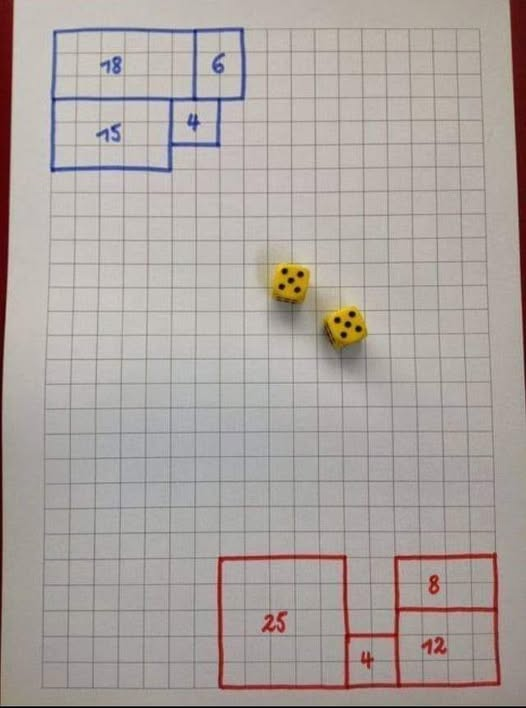
\includegraphics[width=0.45\textwidth]{images/jeu_carre_aire.jpg}
    \end{center}
\end{multicols}

\vspace{-0.7cm}\subsection{Juniper Green}


\begin{Definition}[Multiple et diviseur]
    \vspace{-0.2cm}\begin{multicols}{2}
    On dit qu'un nombre entier est \acc{multiple} d'un autre nombre entier si le premier nombre est dans la \acc{table de multiplication} du second. \\
       
    \columnbreak

    \textbf{Exemple : }

    $12$ est un \acc{multiple} de $3$ car $12 = 4 \times 3$.
\end{multicols}

    \vspace{-0.75cm}\begin{multicols}{2}
        On dit qu'un nombre entier est un \acc{diviseur} d'un autre nombre entier si on peut \acc{effectuer} la \acc{division} du second nombre par le premier, avec un \acc{reste} nul.  

        \columnbreak

        \textbf{Exemple : }

        $5$ est un \acc{diviseur} de $20$ car \opidiv{20}{5}

        Le reste vaut $0$.
    \end{multicols}
\end{Definition}
\vspace{-0.25cm}\begin{multicols}{2}
\boite{Matériel :}{
\begin{itemize}[itemsep=0em]
    \item Un plateau de jeu composé de : \textbf{un tableau de jeu} et d'\textbf{une pochette plastique}.
    \item Des feutres effaçables.
    \item Une feuille de brouillon
\end{itemize}
}

\columnbreak

\boite{Règles du jeu}{
\begin{itemize}[itemsep=0em]
    \item Le joueur qui commence barre un nombre pair.
    \item Ensuite, chaque joueur, à tour de rôle, barre un nombre parmi les \textbf{multiples} ou les \textbf{diviseurs} du nombre barré par son adversaire.
\end{itemize}
}
\end{multicols}
\vspace{-0.5cm}\boite{Objectif : }{
    \textbf{Un joueur est déclaré gagnant lorsque son adversaire ne peut plus jouer.}
}

%\newpage 

\boite{Exemple de tour de jeu :}{
\begin{itemize}
    \item Si le joueur A barre le 12, le joueur B doit barrer un multiple ou un diviseur de 12. Il n'y a pas de multiple de 12 sur le plateau, il a donc le choix entre les diviseurs de 12 : 1 ; 2 ; 3 ; 4 et 6. Supposons que le joueur B barre le 3.
    \item Le joueur A peut alors barrer le 1, le 6, le 9, le 15 ou le 18. Supposons qu'il barre le 9.
    \item Le joueur B ne peut plus barrer que le 1 ou le 18. Supposons qu'il barre le 1.
    \item Le joueur A peut alors barrer n'importe quel nombre restant sur le plateau. Supposons qu'il barre le 19. Le joueur B ne peut plus jouer. Le joueur A est déclaré gagnant.
\end{itemize}
}

%\vspace{-1cm}\section*{Plateaux de jeux}

\begin{multicols}{2}
\boite{Niveau 1 :}{\begin{center}
\begin{tabular}{|c|c|c|c|c|}
\hline
1 & 2 & 3 & 4 \\
\hline
5 & 6 & 7 & 8 \\
\hline
9 & 10 & 11 & 12 \\
\hline
13 & 14 & 15 & 16 \\
\hline
17 & 18 & 19 & 20 \\
\hline
\end{tabular}
\end{center}
}
\boite{Niveau 2 :}{
\begin{center}
\begin{tabular}{|c|c|c|c|c|}
\hline
1 & 2 & 3 & 4 & 5 \\
\hline
6 & 7 & 8 & 9 & 10 \\
\hline
11 & 12 & 13 & 14 & 15 \\
\hline
16 & 17 & 18 & 19 & 20 \\
\hline
21 & 22 & 23 & 24 & 25 \\
\hline
26 & 27 & 28 & 29 & 30 \\
\hline
31 & 32 & 33 & 34 & 35 \\
\hline
36 & 37 & 38 & 39 & 40 \\
\hline
\end{tabular}
\end{center}
}

\columnbreak

\boite{Niveau 3 :}{
\begin{center}
\begin{tabular}{|c|c|c|c|c|c|c|c|c|c|}
\hline
1 & 2 & 3 & 4 & 5 & 6 & 7 & 8 & 9 & 10 \\
\hline
11 & 12 & 13 & 14 & 15 & 16 & 17 & 18 & 19 & 20 \\
\hline
21 & 22 & 23 & 24 & 25 & 26 & 27 & 28 & 29 & 30 \\
\hline
31 & 32 & 33 & 34 & 35 & 36 & 37 & 38 & 39 & 40 \\
\hline
41 & 42 & 43 & 44 & 45 & 46 & 47 & 48 & 49 & 50 \\
\hline
51 & 52 & 53 & 54 & 55 & 56 & 57 & 58 & 59 & 60 \\
\hline
61 & 62 & 63 & 64 & 65 & 66 & 67 & 68 & 69 & 70 \\
\hline
71 & 72 & 73 & 74 & 75 & 76 & 77 & 78 & 79 & 80 \\
\hline
81 & 82 & 83 & 84 & 85 & 86 & 87 & 88 & 89 & 90 \\
\hline
91 & 92 & 93 & 94 & 95 & 96 & 97 & 98 & 99 & 100 \\
\hline
\end{tabular}
\end{center}
}
\end{multicols} % Inclusion de l'énoncé

\newpage 

\subsection{Multiplicato}

\begin{multicols}{2}
\boite{Matériel :}{
\begin{itemize}
    \item La feuille de jeu
    \item Un stylo rouge
    \item Un stylo bleu
\end{itemize}
}

\columnbreak

\boite{But :}{
Faire le plus possible d'alignements d'au moins trois nombres en ligne ou en colonne, contigus ou non, en les entourant de sa couleur.
}
\end{multicols}

\begin{multicols}{2}
\boite{Nombre de joueurs :}{
2 joueurs.
}

\columnbreak

\boite{Mécanisme :}{
Un coup est valide quand le joueur annonce un produit égal au nombre qu'il a choisi sur la grille. Les produits doivent se situer dans la limite de 10 x 10 pour le niveau 1 et de 12 x 12 pour le niveau 2.\\

Lien vers la démo : \href{https://jeux2maths.fr/multiplicato/}{https://jeux2maths.fr/multiplicato/}
}
\end{multicols}

\begin{multicols}{2}
\boite{Déroulement d'une partie :}{
\begin{itemize}
    \item Un joueur se munit d'un stylo rouge, l'autre d'un stylo bleu. La feuille de jeu est placée entre les joueurs.
    \item L'adversaire impose au joueur de choisir un nombre dans une table de multiplication pour laquelle il existe un produit disponible sur la grille.
    \item Le joueur annonce le produit correspondant au nombre qu'il choisit sur la grille, entoure ce nombre lorsque son adversaire a validé le choix et écrit le produit dans sa colonne sur la feuille de jeu. Il impose à son tour une table de multiplication dans laquelle son adversaire devra jouer.
    \item Si l'adversaire propose une table pour laquelle il n'existe plus de nombre disponible sur la grille, le joueur entoure un nombre de son choix.
    \item Si le joueur commet une erreur dans son produit, il ne peut jouer, et c'est alors l'adversaire qui entoure un nombre de son choix.
    \item La partie se termine quand tous les nombres sont entourés sur la grille.
\end{itemize}
}

\columnbreak

\boite{Scores :}{
Les points sont comptés à l'issue de la partie.
\begin{itemize}
    \item Un alignement de 3 nombres dans une couleur vaut 1 point.
    \item Un alignement de 4 nombres dans une couleur vaut 3 points.
    \item Un alignement de 5 nombres dans une couleur vaut 10 points.
\end{itemize}
Le vainqueur est le joueur qui totalise le plus de points à l'issue de la partie.

Remarque : on peut également comptabiliser les alignements effectués en diagonale, mais le comptage s'avère alors difficile pour la majeure partie des élèves.
}
\end{multicols} % Inclusion de la solution



%\newpage 
\section{La course aux nombres}

\section{La course aux nombres}

%\vspace{-0.2cm}

\begin{Activite}[La course aux nombres]

    La \acc{course aux nombres} désigne un jeu qui se joue en \acc{tour par tour} et \acc{par équipe} permettant de réaliser des \acc{opérations de nombres décimaux} à l'aide une \acc{frise graduée}.


    %\vspace{-0.3cm}
    \begin{multicols}{2}

        \boite{Fonctionnement d'un tour :}{
            \vspace{-0.2cm}\begin{enumerate}%[label=\faPen]
                \item Un joueur lance trois dés à $10$ faces.
                \item Un deuxième joueur complète la fiche d'avancement avec le \acc{nombre formé}.
                \item L'équipe \acc{ajoute} ce nombre à son résultat précédent sur la fiche d'avancement.
                \item L'équipe avance son curseur sur la frise pour correspondre à ce résultat. 
                \item S'il y a un \acc{événement} sur la case d'arrivée, l'équipe effectue l'action\\ \acc{1 événement maximum par tour}. 
            \end{enumerate}
        }

        \columnbreak
        \begin{center}
            \begin{tikzpicture}
                % Inclusion de l'image des dés
                \node (image) at (0,0) {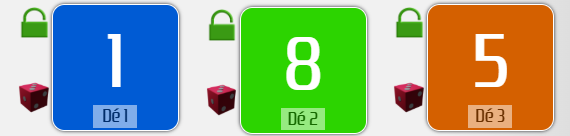
\includegraphics[width=5cm]{images/image_des.png}};
                
                % Positions des nombres formés
                %\node (n1) at (-1.6,-1.3) {\Huge \textbf{1}};
                \node (n12) at (0,-1.5) {\Huge $\mathbf{1,85}$};
                \node (n22) at (2.5,-1.5) {( nombre formé )};
                
                %\node (n23) at (1.2,-1.3) {\Huge \textbf{2 3}};
                
                % Flèches reliant les dés aux chiffres correspondants
                \draw[->, thick] (-1.5,-0.55) -- (n12.north west);
                \draw[->, thick] (0.15,-0.55) -- (0.15,-1);
                \draw[->, thick] (1.8,-0.55) -- (n12.north east);
            \end{tikzpicture}
        \end{center}
        \boite{Les événements possibles :}{ 
            % Définition de la commande pour afficher un rectangle coloré à hauteur de texte
            \newcommand{\rectangle}[1]{%
                \tikz[baseline=-0.5ex] \node[draw, fill=#1, minimum width=1em, minimum height=1em, inner sep=0pt] {};%
            }
            \vspace{-0.2cm}\begin{itemize}[label=\textbf{Type}]
                \item \textbf{R}\  \rectangle{green!85!black} : \acc{Jouer immédiatement un nouveau tour}.
                \item \textbf{C}\   \rectangle{green!85!white} : \acc{Avancer d'une unité}.
                \item \textbf{M}\   \rectangle{red!85!black} : \acc{Reculer d'une unité}.
                \item \textbf{D}\   \rectangle{blue!50} : \acc{Résoudre un défi en 30 secondes}.
                \item \textbf{E}\ Toute erreur de calcul est pénalisée par un événement : \acc{Reculer d'une unité}.
            \end{itemize}
        }
    \end{multicols}%
    \vspace{-0.35cm}\boite{Fin de partie si :}{
        \begin{multicols}{2}
            \begin{itemize}[itemsep=0em,label=$\bullet$]
                \item Une équipe arrive au bout de la frise.
                \item Le temps est écoulé. 
            \end{itemize}

                \columnbreak

            \begin{itemize}[itemsep=0em,label=$\bullet$]
                \item Une équipe complète sa fiche.
            \end{itemize}
            \vspace{-0.25cm}L'équipe qui arrive le plus loin \acc{gagne}.
        \end{multicols}
    }
\end{Activite}%

\newpage


\subsection{Informations sur la frise}% Définition des constantes

\boite{Matériel :}{
    \vspace{-0.2cm}\begin{multicols}{2}
        \begin{itemize}[label=\bcoutil]
        \item Trois dés à $10$ faces ou un \href{https://www.ma-calculatrice.fr/des-virtuels-simulateur?nbre_des=3&de_couleurs_1=005BD4&de_min_1=0&de_max_1=9&de_couleurs_2=2CD400&de_min_2=0&de_max_2=9&de_couleurs_3=D46000&de_min_3=0&de_max_3=9&de_couleurs_4=000000&de_min_4=1&de_max_4=6&de_couleurs_5=000000&de_min_5=1&de_max_5=6&de_couleurs_6=000000&de_min_6=1&de_max_6=6&de_couleurs_7=000000&de_min_7=1&de_max_7=6&de_couleurs_8=000000&de_min_8=1&de_max_8=6&de_couleurs_9=000000&de_min_9=1&de_max_9=6&de_couleurs_10=000000&de_min_10=1&de_max_10=6&de_couleurs_11=000000&de_min_11=1&de_max_11=6&de_couleurs_12=000000&de_min_12=1&de_max_12=6}{simulateur}.
        \item Des \acc{curseurs} représentant chaque équipe.
        \item Des cartes \acc{défis}.
        \item Des cartes \acc{rôle}.
        
        \columnbreak

        \item Une calculatrice pour l'équipe d'arbitrage.
        \item Une \acc{frise graduée}.
        \item Une \acc{fiche équipe}.
        \item Un chronomètre : \phantom{a}\hfill \overlaychrono{15} \hfill \phantom{a}
        \end{itemize}
    \end{multicols}
}
\def\bandwidth{4.5} % Largeur d'une bande en cm
\def\bandheight{25} % Hauteur d'une bande en cm
\def\languette{0.8}
\def\echellegraphique{10}
\def\nombremax{50}
\edef\nombrepage{\fpeval{round(\nombremax/(3*2.5),0)}}
\def\reste{1}
\begin{multicols}{2}
\begin{itemize}[label=$\bullet$]
    \item La frise suivante est à découper. 
    \item Il suffit ensuite de coller les languettes, pour assembler la frise.
    \item La frise est composée de $\num{\fpeval{(\nombrepage-\reste)*3+2}}$ morceaux répartis sur $\num{\nombrepage}$ pages.
    \item Longueur totale : $\num{\fpeval{(\bandheight * (\nombrepage - \reste) * 3 +\bandheight * 2 )  / 100}}$ m.
\end{itemize}

\columnbreak

La répartition des \acc{événements} est générée comme suit : 
\begin{center}
    \begin{tcbtab}{c|c|c|c|c}
        Type & R & C & M & D \\
        \hline
        Probabilité & $\frac{1}{6}$ & $\frac{1}{6}$ & $\frac{1}{6}$ & $\frac{1}{2}$\\
    \end{tcbtab}
\end{center}
\end{multicols}

\begin{Exemple}[Fonctionnement d'un tour de jeu]
    \vspace{-0.3cm}\begin{multicols}{2}
        \begin{enumerate}[itemsep=0em]
            \item L'équipe commence son tour à l'\acc{abscisse} $\num{7.45}$.
            \item Les élèves obtiennent, \acc{dans l'ordre} $4$, $1$ et $6$. 
            \item Le responsable complète la \acc{fiche d'avancement} avec le nombre $\num{4.16}$.
            \item L'équipe complète le résultat par $\num{7.45} + \num{4.16} = \num{\fpeval{7.45+4.16}}$.
            \item Le résultat est validé par l'équipe arbitre qui a le droit d'utiliser la calculatrice. 
            \item L'équipe tombe sur une case notée \frquote{Défi}. \\
            L'équipe pioche une carte \frquote{défi} de difficulté $2$ et répond à la question correctement.
            \item Les arbitres valident la solution. L'équipe avance de $2$ unités supplémentaires et note cette étape dans la \acc{fiche d'avancement}.
        \end{enumerate}

    \end{multicols}

    \begin{tcbtab}[Extrait de la fiche d'avancement]{c|c|c|c|c|c}
        %$\phantom{\dfrac{\dfrac{1}{10}}{\dfrac{1}{10}}}$ Tour $\phantom{\dfrac{\dfrac{1}{10}}{\dfrac{1}{10}}}$ & $1$ & $\dfrac{1}{10}$ & $\dfrac{1}{100}$ & Nombre formé & Résultat \\
        Action \no & Dé \no 1 & Dé \no 2 & Dé \no 3 & Nombre formé & Résultat \\
        \hline
        \repsim[1cm]{}  & \repsim{X} & \repsim{X} & \repsim{X} & \repsim[3cm]{X} & \repsim[6cm]{$\num{7.45}$}\\
        \hline
        \repsim[1cm]{}  & \repsim{$4$} & \repsim{$1$} & \repsim{$6$} & \repsim[3cm]{$\num{4.16}$} & \repsim[6cm]{$\num{7.45} + \num{4.16} = \num{\fpeval{7.45+4.16}}$}\\
        \hline
        \repsim[1cm]{}  & \repsim{X} & \repsim{X} & \repsim{X} & \repsim[3cm]{2} & \repsim[6cm]{$\num{\fpeval{7.45+4.16}} + 2 = \num{\fpeval{7.45+4.16+2}}$}\\
        \hline
        
    \end{tcbtab}

\end{Exemple}

\newpage



\section{Le matériel de la course aux nombres}

\subsection{Cartes de rôles}
\newcommand{\rolecard}[2]{%
  \begin{tcolorbox}[
    enhanced,
    width=7cm,
    colback=blue!10!white,
    colframe=blue!50!black,
    boxrule=1mm,
    arc=5mm,
    drop shadow={xshift=2mm,yshift=-2mm,opacity=0.5},
    fontupper=\small,
    fonttitle=\bfseries\Large,
    coltitle=white,
    colbacktitle=blue!50!black,
    title={#1},
    attach boxed title to top center={yshift=-3mm},
    boxed title style={
      sharp corners,
      boxrule=0mm,
      interior style={left color=blue!50!black, right color=blue!30!white}
    },
    overlay={%
      % Petit cercle en haut à gauche
      \draw[fill=yellow!80!orange, draw=yellow!50!red, line width=0.5mm] 
        ([xshift=-2mm,yshift=-2mm]frame.north west) circle (3mm);
      % Petit cercle en haut à droite
      \draw[fill=yellow!80!orange, draw=yellow!50!red, line width=0.5mm] 
        ([xshift=2mm,yshift=-2mm]frame.north east) circle (3mm);
      % Une étoile décorative centrée en haut
      \node[rotate=15, scale=1.2] at ([yshift=-1cm]frame.north) {\faStar};
    }
  ]
    #2
  \end{tcolorbox}
}



\begin{multicols}{2}
    \rolecard{Joueur 1}{
        \begin{center}\acc{Responsable des dés}\end{center}
        \begin{itemize}[label=\faPen]
            \item Lance trois dés à 10 faces au début de chaque tour.
            \item S'il les lance plusieurs fois d'affilée, le tour de l'équipe est annulé.
            \item Participe aux calculs en collaboration avec l'équipe.
            \item Participe à la résolution de problèmes.
        \end{itemize}
    }

    \rolecard{Joueur 2}{
        \begin{center}\acc{Responsable de la fiche}\end{center}
        \begin{itemize}[label=\faPen]
            \item Note le nombre formé en utilisant les valeurs obtenues avec les dés.
            \item Ajoute ce nombre au résultat précédent.
            \item Participe aux calculs en collaboration avec l'équipe.
            \item Participe à la résolution de problèmes.        
        \end{itemize}
    }
\end{multicols}

\vspace{3cm}

\begin{multicols}{2}

    \rolecard{Joueur 3}{
        \begin{center}\acc{Responsable du curseur}\end{center}
        \begin{itemize}[label=\faPen]
            \item Déplace le curseur sur la frise graduée en fonction du résultat.
            \item Vérifie si l'équipe atterrit sur un événement particulier.
            \item Participe aux calculs en collaboration avec l'équipe.
            \item Participe à la résolution de problèmes.
        \end{itemize}
    }

    \rolecard{Joueur 4}{
        \begin{center}\acc{Responsable de la communication}\end{center}
        \begin{itemize}[label=\faPen]
            \item Informe l'équipe des règles et des événements déclenchés.
            \item Vérifie et annonce les actions à réaliser en fonction des cases atteintes.
            \item Participe aux calculs en collaboration avec l'équipe.
            \item Participe à la résolution de problèmes.
        \end{itemize}
    }
\end{multicols}

\newpage

\begin{multicols}{2}
    \rolecard{Arbitre}{
        \begin{center}\phantom{a}\end{center}
        \begin{itemize}[label=\faPen]
            \item Valide les calculs des équipes en utilisant la calculatrice.
            \item Chronomètre les défis ( 30 secondes à 1 minute ).
            \item Peut \acc{mettre en pause} la partie à tout moment.
            \item Peut \acc{annuler une action} s'il estime que l'équipe n'est pas correcte. \\ ( triche, antijeu, moqueries...)
            \item Demande l'intervention du professeur en cas de problème.
        \end{itemize}
    }

    \columnbreak

    \rolecard{Arbitre}{
        \begin{center}\phantom{a}\end{center}
        \begin{itemize}[label=\faPen]
            \item Valide les calculs des équipes en utilisant la calculatrice.
            \item Chronomètre les défis ( 30 secondes à 1 minute ).
            \item Peut \acc{mettre en pause} la partie à tout moment.
            \item Peut \acc{annuler une action} s'il estime que l'équipe n'est pas correcte. \\ ( triche, antijeu, moqueries...)
            \item Demande l'intervention du professeur en cas de problème.
        \end{itemize}
    }
\end{multicols}

% Commande pour dessiner une case à cocher vide.
\newcommand{\hereismycheckbox}{%
  \tikz[scale=0.8] \draw[thick] (0,0) rectangle (0.4,0.4);%
}

\begin{center}
    % Le tableau comporte une première colonne pour le libellé puis 6 colonnes (3 pour chaque équipe)
    \begin{tcbtab}{p{5cm} |*{3}{>{\centering\arraybackslash}p{1.5cm}} |*{3}{>{\centering\arraybackslash}p{1.5cm}}}
      \hline
      \multirow{2}{*}{\centering\textbf{Infractions}} & \multicolumn{3}{c|}{\textbf{Équipe \no\repsim[1cm]{}}} & \multicolumn{3}{c|}{\textbf{Équipe \no\repsim[1cm]{}}} \\
      \cline{2-7}
      & \textbf{Niv. 1} & \textbf{Niv. 2} & \textbf{Niv. 3} & \textbf{Niv. 1} & \textbf{Niv. 2} & \textbf{Niv. 3} \\
      \hline
      % Exemple de ligne d'infraction avec 3 cases par équipe
      Triche aux dés & \hereismycheckbox & \hereismycheckbox & \hereismycheckbox & \hereismycheckbox & \hereismycheckbox & \hereismycheckbox \\
      \hline
      % Ajoutez ici d'autres infractions
      Retarder l'activité & \hereismycheckbox & \hereismycheckbox & \hereismycheckbox & \hereismycheckbox & \hereismycheckbox & \hereismycheckbox \\
      \hline
      Bavardages excessifs & \hereismycheckbox & \hereismycheckbox & \hereismycheckbox & \hereismycheckbox & \hereismycheckbox & \hereismycheckbox \\
      \hline
      Non-respect des consignes & \hereismycheckbox & \hereismycheckbox & \hereismycheckbox & \hereismycheckbox & \hereismycheckbox & \hereismycheckbox \\
      \hline
      Dégrade le matériel & \hereismycheckbox & \hereismycheckbox & \hereismycheckbox & \hereismycheckbox & \hereismycheckbox & \hereismycheckbox \\
      \hline
      Ne respecte pas l'arbitre & \hereismycheckbox & \hereismycheckbox & \hereismycheckbox & \hereismycheckbox & \hereismycheckbox & \hereismycheckbox \\
      \hline
    \end{tcbtab}
  \end{center}

  Observations : 

  \begin{crep}[extra lines=5]
    \phantom{a}

  \end{crep}

   \vspace{3cm}

\subsection{Fiche d'avancement}

\newpage

\chapitre[
    $\mathbf{6^{\text{ème}}}$% : $\mathbf{6^{\text{ème}}}$,$\mathbf{5^{\text{ème}}}$,$\mathbf{4^{\text{ème}}}$,$\mathbf{3^{\text{ème}}}$,$\mathbf{2^{\text{nde}}}$,$\mathbf{1^{\text{ère}}}$,$\mathbf{T^{\text{Le}}}$,
    ]{
    % : ,Equations
    }{
    Collège% : Collège,Lycée
    }{
    Amadis Jamyn% : Amadis Jamyn,Eugène Belgrand
    }{
    % : ,\tableauPresenteEvalSixieme{}{10},\tableofcontents
    }{
        Fiche d'avancement% : Exercices
    }
\setcounter{tourcounter}{0}
\vspace{-0.8cm}\begin{center}
    \begin{tcbtab}{c|c|c|c|c}
        \'Equipe \no\repsim[1cm]{}& Joueur 1 & Joueur 2 & Joueur 3 & Joueur 4\\
        \hline
        Nom & \repsim[3.3cm]{} & \repsim[3.3cm]{} & \repsim[3.3cm]{} & \repsim[3.3cm]{}\\
        \hline
        Responsable de : & Dés & Fiche d'avancement & Curseur & Communication \\
    \end{tcbtab}
\end{center}
\vspace{-0.8cm}\begin{center}
    \begin{tcbtab}{c|c|c|c|c|c}
        %$\phantom{\dfrac{\dfrac{1}{10}}{\dfrac{1}{10}}}$ Tour $\phantom{\dfrac{\dfrac{1}{10}}{\dfrac{1}{10}}}$ & $1$ & $\dfrac{1}{10}$ & $\dfrac{1}{100}$ & Nombre formé & Résultat \\
        Action \no & Dé \no 1 & Dé \no 2 & Dé \no 3 & Nombre formé & Résultat \\
        \hline
        \repsim[1cm]{}  & \repsim{} & \repsim{} & \repsim{} & \repsim[3cm]{} & \repsim[6cm]{}\\
        \hline
        \repsim[1cm]{}  & \repsim{} & \repsim{} & \repsim{} & \repsim[3cm]{} & \repsim[6cm]{}\\
        \hline
        \repsim[1cm]{}  & \repsim{} & \repsim{} & \repsim{} & \repsim[3cm]{} & \repsim[6cm]{}\\
        \hline
        \repsim[1cm]{}  & \repsim{} & \repsim{} & \repsim{} & \repsim[3cm]{} & \repsim[6cm]{}\\
        \hline
        \repsim[1cm]{}  & \repsim{} & \repsim{} & \repsim{} & \repsim[3cm]{} & \repsim[6cm]{}\\
        \hline
        \repsim[1cm]{}  & \repsim{} & \repsim{} & \repsim{} & \repsim[3cm]{} & \repsim[6cm]{}\\
        \hline
        \repsim[1cm]{}  & \repsim{} & \repsim{} & \repsim{} & \repsim[3cm]{} & \repsim[6cm]{}\\
        \hline
        \repsim[1cm]{}  & \repsim{} & \repsim{} & \repsim{} & \repsim[3cm]{} & \repsim[6cm]{}\\
        \hline
        \repsim[1cm]{}  & \repsim{} & \repsim{} & \repsim{} & \repsim[3cm]{} & \repsim[6cm]{}\\
        \hline
        \repsim[1cm]{}  & \repsim{} & \repsim{} & \repsim{} & \repsim[3cm]{} & \repsim[6cm]{}\\
        \hline
        \repsim[1cm]{}  & \repsim{} & \repsim{} & \repsim{} & \repsim[3cm]{} & \repsim[6cm]{}\\
        \hline
        \repsim[1cm]{}  & \repsim{} & \repsim{} & \repsim{} & \repsim[3cm]{} & \repsim[6cm]{}\\
        \hline
        \repsim[1cm]{}  & \repsim{} & \repsim{} & \repsim{} & \repsim[3cm]{} & \repsim[6cm]{}\\
        \hline
        \repsim[1cm]{}  & \repsim{} & \repsim{} & \repsim{} & \repsim[3cm]{} & \repsim[6cm]{}\\
        \hline
        \repsim[1cm]{}  & \repsim{} & \repsim{} & \repsim{} & \repsim[3cm]{} & \repsim[6cm]{}\\
        \hline
        \repsim[1cm]{}  & \repsim{} & \repsim{} & \repsim{} & \repsim[3cm]{} & \repsim[6cm]{}\\
        \hline
        \repsim[1cm]{}  & \repsim{} & \repsim{} & \repsim{} & \repsim[3cm]{} & \repsim[6cm]{}\\
        \hline
        \repsim[1cm]{}  & \repsim{} & \repsim{} & \repsim{} & \repsim[3cm]{} & \repsim[6cm]{}\\
        \hline
        \repsim[1cm]{}  & \repsim{} & \repsim{} & \repsim{} & \repsim[3cm]{} & \repsim[6cm]{}\\
        \hline
        \repsim[1cm]{}  & \repsim{} & \repsim{} & \repsim{} & \repsim[3cm]{} & \repsim[6cm]{}
    \end{tcbtab}        
\end{center}

\newcommand{\drawGraduations}[3]{%
    % #1: Start value
    % #2: End value
    % #3: Offset value (for continuity)

    % Centièmes graduations (réduction du nombre de graduations)
    \def\scalefactor{1}

    \foreach \x in {#1,0.1,...,#2} {
        \draw[very thick] (0,\x*\scalefactor) -- (0.6, \x*\scalefactor);
    }

    % Dixièmes graduations
    \foreach \x in {#1,1,...,#2} {
        \draw[very thick] (0,\x*\scalefactor) -- (1.5, \x*\scalefactor);
    }

    % Unités graduations et affichage en grand et gras pour les entiers
    \foreach \x in {#1,1,...,\fpeval{#2+0.1}} {
        \draw[very thick] (0,\x*\scalefactor) -- (1.5, \x*\scalefactor);
        \pgfmathsetmacro{\value}{(\x + #3) / 10}
        \pgfmathsetmacro{\semivalue}{(\x + #3 + 5) / 10}
        \pgfmathsetmacro{\semiremainder}{mod(\semivalue,1)}
        \pgfmathsetmacro{\remainder}{mod(\value,1)}
        \ifdim \remainder pt = 0pt
            \node[left, font=\bfseries\LARGE] at (0, \x*\scalefactor) {\fpeval{\value}};
        \fi
        \ifdim \semiremainder pt = 0pt
            \node[left, font=\bfseries\large] at (0, \x*\scalefactor) {\num{\fpeval{\value}}};
        \fi
    }

        % Gamification : ajouter des événements aléatoires
        \pgfmathsetmacro{\randomShift}{rnd*4 - 2} % Générer une variation entre -2 et +2
        \pgfmathsetmacro{\eventCount}{int(5 + \randomShift)} % Base 5 événements avec une variation de -2 à +2
        \foreach \i in {1,...,\eventCount} {
        \pgfmathsetmacro{\randY}{random(\fpeval{#1},\fpeval{#2 - 3})}
        \pgfmathrandominteger{\randheight}{1}{2}
        \pgfmathsetmacro{\randX}{0.5*\bandwidth}
        \pgfmathrandominteger{\eventType}{1}{6}
        \def\eventcolor{yellow}
        \def\eventTextColor{black}
        % Définition des labels selon l'événement
        \ifnum\eventType=1
            \def\eventText{R}%Relancer les dés
            \def\eventcolor{green!85!black}
        \fi
        \ifnum\eventType=2
            \def\eventText{D}%Défi}
            \def\eventcolor{blue!35!white}
        \fi
        \ifnum\eventType=3
            \def\eventText{C}%Événement chanceux}
            \def\eventcolor{green!75!white}
        \fi
        \ifnum\eventType=4
            \def\eventText{D}%Défi}
            \def\eventcolor{blue!35!white}
        \fi
        \ifnum\eventType=5
            \def\eventText{M}%Événement malchanceux}
            \def\eventcolor{red!85!black}
            \def\eventTextColor{white}
        \fi
        \ifnum\eventType=6
            \def\eventText{D}%Défi}
            \def\eventcolor{blue!35!white}%green!75!white}
        \fi
        % Dessiner l'événement à une position aléatoire
        \draw[fill=\eventcolor, rounded corners] (\randX, \randY) rectangle ++(2, \randheight+1);

        % Calcul de l'intervalle et placement des labels
        \pgfmathsetmacro{\startY}{\randY}
        \pgfmathsetmacro{\endY}{\randY + \randheight}
        \foreach \y in {\startY, \fpeval{\startY + 1}, ..., \endY} {
            \node at (\randX + 1, \y + 0.5) {\LARGE{\textbf{\color{\eventTextColor}\eventText}}};
        }
    }
    
    % Languette de collage pour lier à la frise suivante
    \draw[thick, fill=gray!30] (0, \bandheight) rectangle (\bandwidth, \bandheight + \languette);
    \node[above, font=\small] at (\bandwidth/2, \bandheight + \languette / 10) {Languette de collage};
}





\subsection{Les curseurs}


\vspace{1.5cm}\begin{center}
    \curseur{blue}{1} \hspace{1cm} \curseur{red}{2} \hspace{1cm} \curseur{green}{3}
\end{center}

\vspace{1.5cm}\begin{center}
    \curseur{yellow}{4} \hspace{1cm} \curseur{purple}{5}
\end{center}

\subsection{Tutoriel}

\newpage

\input{tuto_frise.tex}

\newpage

\subsection{La frise}

\newpage

\begin{tikzpicture}[x=1cm, y=1cm,xshift=-1cm]

% Dessin de la première bande
\begin{scope}[shift={(-1,0)}]
    \draw[thick] (0,0) rectangle (\bandwidth, \bandheight);
    \clip (-1.2,-0.5) rectangle (\bandwidth, \bandheight+\languette+1);
    \drawGraduations{0}{25}{0}
\end{scope}

% Dessin de la deuxième bande (avec continuité des nombres)
\begin{scope}[shift={(1*\bandwidth + 1,0)}]
    \draw[thick] (0,0) rectangle (\bandwidth, \bandheight);
    \clip (-1.2,-0.5) rectangle (\bandwidth, \bandheight+\languette+1);
    \drawGraduations{0}{25}{25}
\end{scope}

% Dessin de la troisième bande (avec continuité des nombres)
\begin{scope}[shift={(2*\bandwidth + 3,0)}]
    \draw[thick] (0,0) rectangle (\bandwidth, \bandheight);
    \clip (-1.2,-0.5) rectangle (\bandwidth, \bandheight+\languette+1);
    \drawGraduations{0}{25}{50}
\end{scope}

\end{tikzpicture}

\newpage

\begin{tikzpicture}[x=1cm, y=1cm,xshift=-1cm]
% Dessin de la première bande
\begin{scope}[shift={(-1,0)}]
    \draw[thick] (0,0) rectangle (\bandwidth, \bandheight);
    \clip (-1.2,-0.5) rectangle (\bandwidth, \bandheight+\languette+1);
    \drawGraduations{0}{25}{75}
\end{scope}

% Dessin de la deuxième bande (avec continuité des nombres)
\begin{scope}[shift={(1*\bandwidth + 1,0)}]
    \draw[thick] (0,0) rectangle (\bandwidth, \bandheight);
    \clip (-1.2,-0.5) rectangle (\bandwidth, \bandheight+\languette+1);
    \drawGraduations{0}{25}{100}
\end{scope}

% Dessin de la troisième bande (avec continuité des nombres)
\begin{scope}[shift={(2*\bandwidth + 3,0)}]
    \draw[thick] (0,0) rectangle (\bandwidth, \bandheight);
    \clip (-1.2,-0.5) rectangle (\bandwidth, \bandheight+\languette+1);
    \drawGraduations{0}{25}{125}
\end{scope}

\end{tikzpicture}

\newpage

\begin{tikzpicture}[x=1cm, y=1cm,xshift=-1cm]
% Dessin de la première bande
\begin{scope}[shift={(-1,0)}]
    \draw[thick] (0,0) rectangle (\bandwidth, \bandheight);
    \clip (-1.2,-0.5) rectangle (\bandwidth, \bandheight+\languette+1);
    \drawGraduations{0}{25}{150}
\end{scope}

% Dessin de la deuxième bande (avec continuité des nombres)
\begin{scope}[shift={(1*\bandwidth + 1,0)}]
    \draw[thick] (0,0) rectangle (\bandwidth, \bandheight);
    \clip (-1.2,-0.5) rectangle (\bandwidth, \bandheight+\languette+1);
    \drawGraduations{0}{25}{175}
\end{scope}

% Dessin de la troisième bande (avec continuité des nombres)
\begin{scope}[shift={(2*\bandwidth + 3,0)}]
    \draw[thick] (0,0) rectangle (\bandwidth, \bandheight);
    \clip (-1.2,-0.5) rectangle (\bandwidth, \bandheight+\languette+1);
    \drawGraduations{0}{25}{200}
\end{scope}

\end{tikzpicture}

\newpage

\begin{tikzpicture}[x=1cm, y=1cm,xshift=-1cm]
% Dessin de la première bande
\begin{scope}[shift={(-1,0)}]
    \draw[thick] (0,0) rectangle (\bandwidth, \bandheight);
    \clip (-1.2,-0.5) rectangle (\bandwidth, \bandheight+\languette+1);
    \drawGraduations{0}{25}{225}
\end{scope}

% Dessin de la deuxième bande (avec continuité des nombres)
\begin{scope}[shift={(1*\bandwidth + 1,0)}]
    \draw[thick] (0,0) rectangle (\bandwidth, \bandheight);
    \clip (-1.2,-0.5) rectangle (\bandwidth, \bandheight+\languette+1);
    \drawGraduations{0}{25}{250}
\end{scope}

% Dessin de la troisième bande (avec continuité des nombres)
\begin{scope}[shift={(2*\bandwidth + 3,0)}]
    \draw[thick] (0,0) rectangle (\bandwidth, \bandheight);
    \clip (-1.2,-0.5) rectangle (\bandwidth, \bandheight+\languette+1);
    \drawGraduations{0}{25}{275}
\end{scope}

\end{tikzpicture}

\newpage

\begin{tikzpicture}[x=1cm, y=1cm,xshift=-1cm]
% Dessin de la première bande
\begin{scope}[shift={(-1,0)}]
    \draw[thick] (0,0) rectangle (\bandwidth, \bandheight);
    \clip (-1.2,-0.5) rectangle (\bandwidth, \bandheight+\languette+1);
    \drawGraduations{0}{25}{300}
\end{scope}

% Dessin de la deuxième bande (avec continuité des nombres)
\begin{scope}[shift={(1*\bandwidth + 1,0)}]
    \draw[thick] (0,0) rectangle (\bandwidth, \bandheight);
    \clip (-1.2,-0.5) rectangle (\bandwidth, \bandheight+\languette+1);
    \drawGraduations{0}{25}{325}
\end{scope}

% Dessin de la troisième bande (avec continuité des nombres)
\begin{scope}[shift={(2*\bandwidth + 3,0)}]
    \draw[thick] (0,0) rectangle (\bandwidth, \bandheight);
    \clip (-1.2,-0.5) rectangle (\bandwidth, \bandheight+\languette+1);
    \drawGraduations{0}{25}{350}
\end{scope}

\end{tikzpicture}

\newpage

\begin{tikzpicture}[x=1cm, y=1cm,xshift=-1cm]
% Dessin de la première bande
\begin{scope}[shift={(-1,0)}]
    \draw[thick] (0,0) rectangle (\bandwidth, \bandheight);
    \clip (-1.2,-0.5) rectangle (\bandwidth, \bandheight+\languette+1);
    \drawGraduations{0}{25}{375}
\end{scope}

% Dessin de la deuxième bande (avec continuité des nombres)
\begin{scope}[shift={(1*\bandwidth + 1,0)}]
    \draw[thick] (0,0) rectangle (\bandwidth, \bandheight);
    \clip (-1.2,-0.5) rectangle (\bandwidth, \bandheight+\languette+1);
    \drawGraduations{0}{25}{400}
\end{scope}

% Dessin de la troisième bande (avec continuité des nombres)
\begin{scope}[shift={(2*\bandwidth + 3,0)}]
    \draw[thick] (0,0) rectangle (\bandwidth, \bandheight);
    \clip (-1.2,-0.5) rectangle (\bandwidth, \bandheight+\languette+1);
    \drawGraduations{0}{25}{425}
\end{scope}

\end{tikzpicture}

\newpage

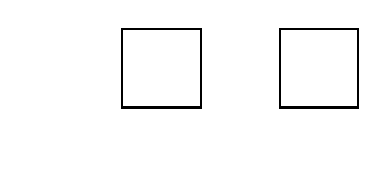
\begin{tikzpicture}[x=1cm, y=1cm,xshift=-1cm]
% Dessin de la première bande
\begin{scope}[shift={(-1,0)}]
    \draw[thick] (0,0) rectangle (\bandwidth, \bandheight);
    \clip (-1.2,-0.5) rectangle (\bandwidth, \bandheight+\languette+1);
    \drawGraduations{0}{25}{450}
\end{scope}

% Dessin de la deuxième bande (avec continuité des nombres)
\begin{scope}[shift={(1*\bandwidth + 1,0)}]
    \draw[thick] (0,0) rectangle (\bandwidth, \bandheight);
    \clip (-1.2,-0.5) rectangle (\bandwidth, \bandheight+\languette+1);
    \drawGraduations{0}{25}{475}
\end{scope}

\end{tikzpicture}


%\newpage

%\section{La grande frise}

%\renewcommand{\drawGraduations}[4]{%
    % #1: Start value
    % #2: End value
    % #3: Offset value (for continuity)

    % Centièmes graduations (réduction du nombre de graduations)
    \def\scalefactor{2}

    \foreach \x in {#1,0.1,...,#2} {
        \draw[very thick] (0,\x*\scalefactor) -- (0.6, \x*\scalefactor);
    }

    % Dixièmes graduations
    \foreach \x in {\fpeval{#1},1,...,#2} {
        \draw[very thick] (0,\fpeval{(\x+#4)*\scalefactor}) -- (1.5, \fpeval{(\x+#4)*\scalefactor});
    }

    % Unités graduations et affichage en grand et gras pour les entiers
    \foreach \x in {\fpeval{#1+#4},1,...,\fpeval{#2+0.1}} {
        \pgfmathsetmacro{\write}{(\x + #3) / (10)}
        \pgfmathsetmacro{\value}{((\x + #3)*\scalefactor) / (10)}
        \pgfmathsetmacro{\semivalue}{((\x + #3 + 5*#4)*\scalefactor)  / (10)}
        \pgfmathsetmacro{\semiremainder}{mod(\semivalue,1)}
        \pgfmathsetmacro{\remainder}{mod(\value,1)}
        \ifdim \remainder pt = 0pt
            \node[left, font=\bfseries\LARGE] at (0, \x*\scalefactor) {\num{\fpeval{\write}}};
            %\draw[very thick] (0,\x*\scalefactor+#4) -- (1.5, \x*\scalefactor+#4);
        \fi
        %\ifdim \semiremainder pt = 0pt
        %    \node[left, font=\bfseries\large] at (0, \x*\scalefactor) {\num{\fpeval{\write}}};
        %    %\draw[very thick] (0,\x*\scalefactor+#4) -- (1.5, \x*\scalefactor+#4);
        %\fi
    }

        % Gamification : ajouter des événements aléatoires
        \pgfmathsetmacro{\randomShift}{rnd*4 - 2} % Générer une variation entre -2 et +2
        \pgfmathsetmacro{\eventCount}{int(\fpeval{(5 + \randomShift)/\scalefactor})} % Base 5 événements avec une variation de -2 à +2
        \foreach \i in {1,...,\eventCount} {
        \pgfmathsetmacro{\randY}{random(\fpeval{#1*\scalefactor},\fpeval{(#2 - 3)*\scalefactor})}
        \pgfmathrandominteger{\randheight}{1}{2}
        \pgfmathsetmacro{\randX}{0.5*\bandwidth}
        \pgfmathrandominteger{\eventType}{1}{4}
        \def\eventcolor{yellow}
        \def\eventTextColor{black}
        % Définition des labels selon l'événement
        \ifnum\eventType=1
            \def\eventText{R}%Relancer les dés
            \def\eventcolor{green!85!black}
        \fi
        \ifnum\eventType=2
            \def\eventText{M}%Événement malchanceux}
            \def\eventcolor{red!85!black}
            \def\eventTextColor{white}
        \fi
        \ifnum\eventType=3
            \def\eventText{C}%Événement chanceux}
            \def\eventcolor{green!75!white}
        \fi
        \ifnum\eventType=4
            \def\eventText{D}%Défi}
            \def\eventcolor{orange}
        \fi
        % Dessiner l'événement à une position aléatoire
        \draw[fill=\eventcolor, rounded corners] (\randX, \randY) rectangle ++(2, \fpeval{(\randheight+1)*\scalefactor});

        % Calcul de l'intervalle et placement des labels
        \pgfmathsetmacro{\startY}{\randY}
        \pgfmathsetmacro{\endY}{\randY + \randheight*\scalefactor}
        \foreach \y in {\startY, \fpeval{\startY + 1*\scalefactor}, ..., \endY} {
            \node at (\randX + 1, \y + 0.5*\scalefactor) {\LARGE{\textbf{\color{\eventTextColor}\eventText}}};
        }
    }
    
    % Languette de collage pour lier à la frise suivante
    \draw[thick, fill=gray!30] (0, \bandheight) rectangle (\bandwidth, \bandheight + \languette);
    \node[above, font=\small] at (\bandwidth/2, \bandheight + \languette / 10) {Languette de collage};
}

La frise suivante est à découper. 

Il suffit ensuite de coller les languettes, pour assembler la frise.

\def\scalefactor{2}
Longueur totale : $\num{\fpeval{10 * \scalefactor * 137.5}}$
\newpage

% Définition des constantes
\def\bandwidth{4.5} % Largeur d'une bande en cm
\def\bandheight{25} % Hauteur d'une bande en cm
\def\languette{0.8}
\begin{tikzpicture}[x=1cm, y=1cm,xshift=-1cm]

% Dessin de la première bande
\begin{scope}[shift={(-1,0)}]
    \draw[thick] (0,0) rectangle (\bandwidth, \bandheight);
    \clip (-1.2,-0.5) rectangle (\bandwidth, \bandheight+\languette+1);
    \drawGraduations{0}{12.5}{0}{0}
\end{scope}

% Dessin de la deuxième bande (avec continuité des nombres)
\begin{scope}[shift={(1*\bandwidth + 1,0)}]
    \draw[thick] (0,0) rectangle (\bandwidth, \bandheight);
    \clip (-1.2,-0.5) rectangle (\bandwidth, \bandheight+\languette+1);
    \drawGraduations{0}{12.5}{12.5}{0.5}
\end{scope}

% Dessin de la troisième bande (avec continuité des nombres)
\begin{scope}[shift={(2*\bandwidth + 3,0)}]
    \draw[thick] (0,0) rectangle (\bandwidth, \bandheight);
    \clip (-1.2,-0.5) rectangle (\bandwidth, \bandheight+\languette+1);
    \drawGraduations{0}{12.5}{25}{0}
\end{scope}

\end{tikzpicture}

\newpage

\begin{tikzpicture}[x=1cm, y=1cm,xshift=-1cm]
% Dessin de la première bande
\begin{scope}[shift={(-1,0)}]
    \draw[thick] (0,0) rectangle (\bandwidth, \bandheight);
    \clip (-1.2,-0.5) rectangle (\bandwidth, \bandheight+\languette+1);
    \drawGraduations{0}{12.5}{37.5}{0.5}
\end{scope}

% Dessin de la deuxième bande (avec continuité des nombres)
\begin{scope}[shift={(1*\bandwidth + 1,0)}]
    \draw[thick] (0,0) rectangle (\bandwidth, \bandheight);
    \clip (-1.2,-0.5) rectangle (\bandwidth, \bandheight+\languette+1);
    \drawGraduations{0}{12.5}{50}{0}
\end{scope}

% Dessin de la troisième bande (avec continuité des nombres)
\begin{scope}[shift={(2*\bandwidth + 3,0)}]
    \draw[thick] (0,0) rectangle (\bandwidth, \bandheight);
    \clip (-1.2,-0.5) rectangle (\bandwidth, \bandheight+\languette+1);
    \drawGraduations{0}{12.5}{67.5}{0.5}
\end{scope}

\end{tikzpicture}

\newpage

\begin{tikzpicture}[x=1cm, y=1cm,xshift=-1cm]

% Dessin de la première bande
\begin{scope}[shift={(-1,0)}]
    \draw[thick] (0,0) rectangle (\bandwidth, \bandheight);
    \clip (-1.2,-0.5) rectangle (\bandwidth, \bandheight+\languette+1);
    \drawGraduations{0}{12.5}{75}{0}
\end{scope}

% Dessin de la deuxième bande (avec continuité des nombres)
\begin{scope}[shift={(1*\bandwidth + 1,0)}]
    \draw[thick] (0,0) rectangle (\bandwidth, \bandheight);
    \clip (-1.2,-0.5) rectangle (\bandwidth, \bandheight+\languette+1);
    \drawGraduations{0}{12.5}{87.5}{0.5}
\end{scope}

% Dessin de la troisième bande (avec continuité des nombres)
\begin{scope}[shift={(2*\bandwidth + 3,0)}]
    \draw[thick] (0,0) rectangle (\bandwidth, \bandheight);
    \clip (-1.2,-0.5) rectangle (\bandwidth, \bandheight+\languette+1);
    \drawGraduations{0}{12.5}{100}{0}
\end{scope}

\end{tikzpicture}

\newpage

\begin{tikzpicture}[x=1cm, y=1cm,xshift=-1cm]
% Dessin de la première bande
\begin{scope}[shift={(-1,0)}]
    \draw[thick] (0,0) rectangle (\bandwidth, \bandheight);
    \clip (-1.2,-0.5) rectangle (\bandwidth, \bandheight+\languette+1);
    \drawGraduations{0}{12.5}{112.5}{0.5}
\end{scope}

% Dessin de la deuxième bande (avec continuité des nombres)
\begin{scope}[shift={(1*\bandwidth + 1,0)}]
    \draw[thick] (0,0) rectangle (\bandwidth, \bandheight);
    \clip (-1.2,-0.5) rectangle (\bandwidth, \bandheight+\languette+1);
    \drawGraduations{0}{12.5}{125}{0}
\end{scope}

% Dessin de la troisième bande (avec continuité des nombres)
\begin{scope}[shift={(2*\bandwidth + 3,0)}]
    \draw[thick] (0,0) rectangle (\bandwidth, \bandheight);
    \clip (-1.2,-0.5) rectangle (\bandwidth, \bandheight+\languette+1);
    \drawGraduations{0}{12.5}{137.5}{0.5}
\end{scope}

\end{tikzpicture}

\newpage

\section{Liste des défis}

\def\points{1}
\def\rdifficulty{3}
\begin{EXO}{}{can6a-2022}

    

	\begin{enumerate}[itemsep=1em, label=\arabic*)]
		\item \itempoint{1}$7 \times 7=$ $\ldots$
		\item \itempoint{1}La moitié de $36$ est : \ldots
		\item \itempoint{1}Complète : \\$19+\ldots =100$ 
		\item \itempoint{1}$3$ cahiers coûtent $9$\,\euro{}.\\ 				 $9$ cahiers coûtent $\ldots$\,\euro{}
		\item \itempoint{1}$2$ h $30$ min $=$ \\ $\ldots$ min
		\item \itempoint{1}Quel est le nombre écrit sous le point d'interrogation ?\\\tikzinclude{gGnt}
		\item \itempoint{1}$32+19=$$\ldots$
		\item \itempoint{1}$18$ élèves se mettent par groupe de $3$. \\ 			  Il y a $\ldots$ groupes.
		\item \itempoint{1}Le tiers de $27$ est :  $\ldots$ 
		\item \itempoint{1}Complète :\\ 				$4+9=\ldots+5$
		\item \itempoint{1}$4{,}4\times 10=$$\ldots$
		\item \itempoint{1}Un film commence à $19$ h $35$ et se termine à $21$ h $15$.\\ 			  Combien de temps a duré le film ?
		\item \itempoint{1}Complète :\\$3=$$\ldots$ quarts
		\item \itempoint{1}Ajoute $25$ min à $7$ h $50$ min.
		\item \itempoint{1}Ajoute un dixième à $2{,}96$.
		\item \itempoint{1}Yann a $30$ billes. Il a $8$ billes de moins que Lou.\\ 				   Lou a $\ldots$ billes.
		\item \itempoint{1}$0{,}2$ kg  $=$   $\ldots$ g
		\item \itempoint{1}Écris en chiffres : \\ 				  Deux-millions-deux-mille 
		\item \itempoint{1}Complète : \\ 				$10$ jours $=$$\ldots$ h
		\item \itempoint{1}Complète : \\ 			  $9$ heures $=$$\ldots$ min
		\item \itempoint{1}Combien faut-il de pièces de $10$ centimes pour avoir $5{,}80$\,\euro{}. \\ 						
		\item \itempoint{1}$0{,}33+0{,}4=$$\ldots$ 
		\item \itempoint{1}Le double de $4{,}8$ est $\ldots$
		\item \itempoint{1}Compléter :\\ $ .... \times 6=36$
	\end{enumerate}
	


\exocorrection


    
\begin{enumerate}[itemsep=1em, label=\arabic*)]
\item $7 \times 7={\color[HTML]{f15929}\boldsymbol{49}}$
\item La moitié de $36$ est $36\div 2={\color[HTML]{f15929}\boldsymbol{18}}$.
\item $100-19={\color[HTML]{f15929}\boldsymbol{81}}$
\item $3$ cahiers coûtent $9$\,\euro{}.\\ 			$3\times3=9$ cahiers coûtent $3\times9={\color[HTML]{f15929}\boldsymbol{27}}$\,\euro{}.
\item $2$ h $30$ min $=2\times 60+ 30$ min $={\color[HTML]{f15929}\boldsymbol{150}}$ min
\item Le nombre écrit sous le point d'interrogation est : ${\color[HTML]{f15929}\boldsymbol{90}}$.
\item $32+19=32+20-1=52-1={\color[HTML]{f15929}\boldsymbol{51}}$
\item Le nombre de groupes est donné par $18\div 3={\color[HTML]{f15929}\boldsymbol{6}}$.
\item Le tiers de $27$ est : $27\div 3={\color[HTML]{f15929}\boldsymbol{9}}$.
\item Le nombre cherché est : $4+9-5={\color[HTML]{f15929}\boldsymbol{8}}$.
\item $4{,}4\times 10={\color[HTML]{f15929}\boldsymbol{44}}$ 
\item Pour aller à $20$ h, il faut $25$ min, et il faut ajouter $1$ heure et $15$ min pour arriver à $21$ h $15$, soit au total ${\color[HTML]{f15929}\boldsymbol{1}}$ h ${\color[HTML]{f15929}\boldsymbol{40}}$ min.
\item $3=\dfrac{12}{4}=12\times \dfrac{1}{4}$, donc ${\color[HTML]{f15929}\boldsymbol{12}}$ quarts $=3$. 
\item Pour aller à $8$ h, il faut $10$ min, et il reste $15$ min à ajouter, ce qui donne ${\color[HTML]{f15929}\boldsymbol{8}}$ h et ${\color[HTML]{f15929}\boldsymbol{15}}$ min.
\item $1$ dixième $=0,1$, d'où $2{,}96+0,1 ={\color[HTML]{f15929}\boldsymbol{3{,}06}}$
\item Yann a $8$ billes de moins que Lou, donc Lou en a $8$ de plus, soit $30+8={\color[HTML]{f15929}\boldsymbol{38}}$ billes.
\item  Comme $1$ kg $=1\,000$ g,  pour passer des "kg" au "g", on multiplie par $1\,000$.\\ 			Comme : $0{,}2\times 1\,000 =200$, alors $0{,}2$ kg$={\color[HTML]{f15929}\boldsymbol{200}}$ g.
\item Deux-millions-deux-mille-deux $=2\,000\,000  + 2\,000 + 2={\color[HTML]{f15929}\boldsymbol{2\,002\,000}}$. 
\item Dans une journée, il y a $24$ heures, donc dans $10$ jours, il y a $10\times 24={\color[HTML]{f15929}\boldsymbol{240}}$ heures.
\item Dans une heure, il y a $60$ minutes, donc dans $9$ heures, il y a $9\times 60={\color[HTML]{f15929}\boldsymbol{540}}$ minutes.
\item Il faut : $5{,}8\div 0,1=5{,}8\times 10={\color[HTML]{f15929}\boldsymbol{58}}$ pièces.
\item  $0{,}33+0{,}4={\color[HTML]{f15929}\boldsymbol{0{,}73}}$
\item Le double de $4{,}8$ est $2\times 4{,}8={\color[HTML]{f15929}\boldsymbol{9{,}6}}$.
\item $ {\color[HTML]{f15929}\boldsymbol{6}} \times 6=36$
\end{enumerate}



\end{EXO}
\def\points{1}
\def\rdifficulty{2}
\begin{EXO}{}{canc3a-2023}

    

\begin{enumerate}[itemsep=1em, label=\arabic*)]
	\item \itempoint{1}$9 \times 4$
	\item \itempoint{1}$36+29$
	\item \itempoint{1}Combien y a-t-il de boules noires ? \\ 
\tikzinclude{ocLB}

	\item \itempoint{1}La moitié de $42$
	\item \itempoint{1}Complète :  $\ldots \times \ldots =35$
	\item \itempoint{1}\Temps{;;;;35;}+ \Temps{;;;;40;}
	\item \itempoint{1}Pour partager $30$ oeufs, combien de boites de  $6$ oeufs dois-je utiliser ? 
	\item \itempoint{1}Écris en chiffres le nombre cinquante-deux-mille-sept.
	\item \itempoint{1}Karole a $12$ ans. \\         Laurent a 5 ans de moins que Karole. Laurent a $\ldots$ ans
	\item \itempoint{1}Donne l'écriture décimale de  $3\times 7$ centièmes.
	\item \itempoint{1}Complète : \,\,\,  $1{,}8+\ldots =10$ 
	\item \itempoint{1}Complète : \,\,\,  $405= \ldots$ dizaines  $\ldots$  unités
	\item \itempoint{1}$25\div 5$
	\item \itempoint{1}Si $2$ cahiers coûtent $8$\,\euro{}, alors $8$ cahiers coûtent  $\ldots$\,\euro{}.
	\item \itempoint{1}$92\times 5$
	\item \itempoint{1}Dans $32$ combien de fois $4$ ?
	\item \itempoint{1}Complète : \,\,\, $7$ centaines et  $\ldots$  dizaines font  $740$.
	\item \itempoint{1}Combien de dixièmes y a-t-il en tout dans $8{,}48$ ?
	\item \itempoint{1}$1{,}93+ 0{,}8$
\end{enumerate}



\exocorrection


    
\begin{enumerate}[itemsep=1em, label=\arabic*)]
\item $9 \times 4={\color[HTML]{f15929}\boldsymbol{36}}$
\item $36+29=36+30-1=66-1={\color[HTML]{f15929}\boldsymbol{65}}$
\item Le nombre de boules noires est donné par : $8\times 3={\color[HTML]{f15929}\boldsymbol{24}}$.
\item La moitié de $42$ est $42\div 2={\color[HTML]{f15929}\boldsymbol{21}}$.
\item Deux réponses possibles (avec des entiers) : \\         ${\color[HTML]{f15929}\boldsymbol{5}}\times {\color[HTML]{f15929}\boldsymbol{7}}=35$\\         ${\color[HTML]{f15929}\boldsymbol{1}}\times {\color[HTML]{f15929}\boldsymbol{35}}=35$ 
\item De $40 \text{ min }$ pour aller à $1$ h, il faut $20$ min, et il reste $15$ min à ajouter.\\         On obtient  ${\color[HTML]{f15929}\boldsymbol{1}}$ h et ${\color[HTML]{f15929}\boldsymbol{15}}$ min.
\item Le nombre de boites est donné par $30\div 6={\color[HTML]{f15929}\boldsymbol{5}}$.
\item cinquante-deux-mille-sept = $52\,000$ + 7 = ${\color[HTML]{f15929}\boldsymbol{52\,007}}$ 
\item Puisque Laurent a 5 ans de moins que Karole, son âge est  : $12-5={\color[HTML]{f15929}\boldsymbol{7}}$ {\color[HTML]{f15929}ans}. 
\item $1$ centième $=0,01$, d'où $3\times 7$ centièmes $=3\times 7\times 0,01={\color[HTML]{f15929}\boldsymbol{0.21}}$.
\item Le nombre cherché est donné par : $10-1{,}8={\color[HTML]{f15929}\boldsymbol{8{,}2}}$.
\item $405 = {\color[HTML]{f15929}\boldsymbol{40}}$ dizaines ${\color[HTML]{f15929}\boldsymbol{5}}$ unités
\item $25\div 5={\color[HTML]{f15929}\boldsymbol{5}}$
\item $2$ cahiers coûtent $8$\,\euro{}.\\ $4\times2=8$ cahiers coûtent $4\times8={\color[HTML]{f15929}\boldsymbol{32}}$\,\euro{}.
\item $92\times 5=92\times 10 \div 2=920\div 2={\color[HTML]{f15929}\boldsymbol{460}}$
\item Dans $32$, il y a ${\color[HTML]{f15929}\boldsymbol{8}}$ fois $4$ car $8\times 4=32$.
\item $740 = 7$ centaines et ${\color[HTML]{f15929}\boldsymbol{4}}$ dizaines
\item $8{,}48 = 8$ unités $4$ dixièmes $8$ centièmes.\\Or $1$ unité = $10$ dixièmes donc $8$ unités $= 80$ dixièmes.\\Finalement $8{,}48 = 84$ dixièmes $8$ centièmes.\\Il y a donc ${\color[HTML]{f15929}\boldsymbol{84}}$ dixièmes en tout dans $8{,}48$.
\item $1{,}93+ 0{,}8={\color[HTML]{f15929}\boldsymbol{2{,}73}}$
\end{enumerate}



\end{EXO}
\def\points{1}
\def\rdifficulty{1}
\begin{EXO}{}{canc3a}

    
\begin{multicols}{2}
\begin{enumerate}[itemsep=1em, label=\arabic*)]
	\item \itempoint{1}\begin{minipage}[t]{\linewidth} $22+13$ \end{minipage}
	\item \itempoint{1}\begin{minipage}[t]{\linewidth} $65-32$ \end{minipage}
	\item \itempoint{1}\begin{minipage}[t]{\linewidth} $17+25$ \end{minipage}
	\item \itempoint{1}\begin{minipage}[t]{\linewidth} $83-25$ \end{minipage}
	\item \itempoint{1}\begin{minipage}[t]{\linewidth} $3\times 1\,000 + 6\times 10 + 5\times 100$ \end{minipage}
	\item \itempoint{1}\begin{minipage}[t]{\linewidth} $2{,}2+3$ \end{minipage}
	\item \itempoint{1}\begin{minipage}[t]{\linewidth} $1{,}4+1{,}16$ \end{minipage}
	\item \itempoint{1}\begin{minipage}[t]{\linewidth} $5{,}63-2{,}2$ \end{minipage}
	\item \itempoint{1}\begin{minipage}[t]{\linewidth} $6{,}1-4{,}5$ \end{minipage}
	\item \itempoint{1}\begin{minipage}[t]{\linewidth} J'ai $18$ ans. Je suis $2$ fois plus âgé que Joachim.\\Quel âge a Joachim ? \end{minipage}
	\item \itempoint{1}\begin{minipage}[t]{\linewidth} Léa a $17$ ans. Sa sœur a $5$ ans.\\Quelle est leur différence d'âge ? \end{minipage}
	\item \itempoint{1}\begin{minipage}[t]{\linewidth} Joachim a couru $2$ séquences de $10$ minutes. Combien de minutes a-t-il couru en tout ? \end{minipage}
	\item \itempoint{1}\begin{minipage}[t]{\linewidth} $\ldots - 3=2{,}2$ \end{minipage}
	\item \itempoint{1}\begin{minipage}[t]{\linewidth} $5 \times 6$ \end{minipage}
	\item \itempoint{1}\begin{minipage}[t]{\linewidth} $6 \times 4$ \end{minipage}
	\item \itempoint{1}\begin{minipage}[t]{\linewidth} On a coupé $4{,}1$ cm d'une ficelle qui en faisait $7{,}2$.\\Combien de centimètres en reste-t-il ? \end{minipage}
	\item \itempoint{1}\begin{minipage}[t]{\linewidth} \tikzinclude{TIsR}\end{minipage}
	\item \itempoint{1}\begin{minipage}[t]{\linewidth} $8 \times 7$ \end{minipage}

	\item \itempoint{1}\begin{minipage}[t]{\linewidth} $\ldots \times 20=190$ \end{minipage}
	\item \itempoint{1}\begin{minipage}[t]{\linewidth} $3$ kg de fraises coûtent $22{,}5$\,\euro{}, combien coûtent $12$ kg de fraises ? \end{minipage}
	\item \itempoint{1}\begin{minipage}[t]{\linewidth} $\ldots \times 4=40$ \end{minipage}
	\item \itempoint{1}\begin{minipage}[t]{\linewidth} Le diamètre d'un cercle de $60$ unités de rayon. \end{minipage}
	\item \itempoint{1}\begin{minipage}[t]{\linewidth} Le film a commencé à $20$ h $30$. Il s'est terminé à $22$ h $25$.\\ Combien de minutes a-t-il duré ? \end{minipage}
	\item \itempoint{1}\begin{minipage}[t]{\linewidth} En $24$ minutes, un manège fait $27$ tours.\\En $8$ minutes il fait \ldots tours. \end{minipage}
\end{enumerate}
\end{multicols}



\exocorrection


    \begin{multicols}{2}

\begin{enumerate}[itemsep=1em, label=\arabic*)]
\item \begin{minipage}[t]{\linewidth}$22+13=35$\end{minipage}
\item \begin{minipage}[t]{\linewidth}$65-32=33$\end{minipage}
\item \begin{minipage}[t]{\linewidth}$17+25=42$\end{minipage}
\item \begin{minipage}[t]{\linewidth}$83-25=58$\end{minipage}
\item \begin{minipage}[t]{\linewidth}$3\times 1\,000 + 6\times 10 + 5\times 100 =3\,560$\end{minipage}
\item \begin{minipage}[t]{\linewidth}$2{,}2+3=5{,}2$\end{minipage}
\item \begin{minipage}[t]{\linewidth}$1{,}4+1{,}16=2{,}56$\end{minipage}
\item \begin{minipage}[t]{\linewidth}$5{,}63-2{,}2=3{,}43$\end{minipage}
\item \begin{minipage}[t]{\linewidth}$6{,}1-4{,}5=1{,}6$\end{minipage}
\item \begin{minipage}[t]{\linewidth}L'âge de Joachim est : $18 \div 2=9$ ans.\end{minipage}
\item \begin{minipage}[t]{\linewidth}La différence d'âge entre Léa et sa sœur est : $17-5=12$ ans.\end{minipage}
\item \begin{minipage}[t]{\linewidth}Joachim a couru : $2 \times 10=20$ minutes.\end{minipage}
\item \begin{minipage}[t]{\linewidth}${\color[HTML]{f15929}\boldsymbol{5{,}2}} - 3=2{,}2$\end{minipage}
\item \begin{minipage}[t]{\linewidth}$5 \times 6=30$\end{minipage}
\item \begin{minipage}[t]{\linewidth}$6 \times 4=24$\end{minipage}
\item \begin{minipage}[t]{\linewidth}$7{,}2-4{,}1=3{,}1$\end{minipage}
\item \begin{minipage}[t]{\linewidth}${\color[HTML]{f15929}\boldsymbol{3{,}5}} + 2{,}4=5{,}9$\end{minipage}
\item \begin{minipage}[t]{\linewidth}$7 \times 8=56$\end{minipage}
\item \begin{minipage}[t]{\linewidth}Le périmètre mesure : $3 \times 5{,}3$ cm $=15{,}9$ cm.\end{minipage}
\item \begin{minipage}[t]{\linewidth}${\color[HTML]{f15929}\boldsymbol{9{,}5}} \times 20=190$\end{minipage}
\item \begin{minipage}[t]{\linewidth}$12$ kg de fraises coûtent : $22{,}5 \times 4 = 90$\,\euro{}.\end{minipage}
\item \begin{minipage}[t]{\linewidth}${\color[HTML]{f15929}\boldsymbol{10}} \times 4=40$\end{minipage}
\item \begin{minipage}[t]{\linewidth}Le diamètre est le double du rayon : $2 \times 60 = 120$\end{minipage}
\item \begin{minipage}[t]{\linewidth}Le film a duré $1$ h $55$ min soit $115$ minutes.\end{minipage}
\item \begin{minipage}[t]{\linewidth}En $3$ fois moins de temps, ce manège fait $3$ fois moins de tours, soit : $27$ tours $\div 3=9$ tours.\end{minipage}
\end{enumerate}
\end{multicols}



\end{EXO}

\newpage

\rdexocorrection{0}

\newpage

\section{Cartes des défis}

\mescartes{red}{Q.3.1}{$7 \times 7=$ $\ldots$}{S.3.1}{$7 \times 7={\color[HTML]{f15929}\boldsymbol{49}}$}%
\mescartes{red}{Q.3.2}{La moitié de $36$ est : \ldots}{S.3.2}{La moitié de $36$ est $36\div 2={\color[HTML]{f15929}\boldsymbol{18}}$.}%
\vspace{1cm}
\mescartes{red}{Q.3.3}{Complète : \\$19+\ldots =100$}{S.3.3}{$100-19={\color[HTML]{f15929}\boldsymbol{81}}$}%
\mescartes{red}{Q.3.4}{$3$ cahiers coûtent $9$\,\euro{}.\\                               $9$ cahiers coûtent $\ldots$\,\euro{}}{S.3.4}{$3$ cahiers coûtent $9$\,\euro{}.\\                      $3\times3=9$ cahiers coûtent $3\times9={\color[HTML]{f15929}\boldsymbol{27}}$\,\euro{}.}%       
\vspace{1cm}
\mescartes{red}{Q.3.5}{$2$ h $30$ min $=$ \\ $\ldots$ min}{S.3.5}{$2$ h $30$ min $=2\times 60+ 30$ min $={\color[HTML]{f15929}\boldsymbol{150}}$ min}%
\mescartes{red}{Q.3.6}{Quel est le nombre écrit sous le point d'interrogation ?\\\tikzinclude{gGnt}}{S.3.6}{Le nombre écrit sous le point d'interrogation est : ${\color[HTML]{f15929}\boldsymbol{90}}$.}%
\vspace{1cm}
\mescartes{red}{Q.3.7}{$32+19=$$\ldots$}{S.3.7}{$32+19=32+20-1=52-1={\color[HTML]{f15929}\boldsymbol{51}}$}%
\mescartes{red}{Q.3.8}{$18$ élèves se mettent par groupe de $3$. \\                       Il y a $\ldots$ groupes.}{S.3.8}{Le nombre de groupes est donné par $18\div 3={\color[HTML]{f15929}\boldsymbol{6}}$.}%
\vspace{1cm}
\mescartes{red}{Q.3.9}{Le tiers de $27$ est :  $\ldots$}{S.3.9}{Le tiers de $27$ est : $27\div 3={\color[HTML]{f15929}\boldsymbol{9}}$.}%       
\mescartes{red}{Q.3.10}{Complète :\\                            $4+9=\ldots+5$}{S.3.10}{Le nombre cherché est : $4+9-5={\color[HTML]{f15929}\boldsymbol{8}}$.}%
\vspace{1cm}
\mescartes{red}{Q.3.11}{$4{,}4\times 10=$$\ldots$}{S.3.11}{$4{,}4\times 10={\color[HTML]{f15929}\boldsymbol{44}}$}%
\mescartes{red}{Q.3.12}{Un film commence à $19$ h $35$ et se termine à $21$ h $15$.\\                     Combien de temps a duré le film ?}{S.3.12}{Pour aller à $20$ h, il faut $25$ min, et il faut ajouter $1$ heure et $15$ min pour arriver à $21$ h $15$, soit au total ${\color[HTML]{f15929}\boldsymbol{1}}$ h ${\color[HTML]{f15929}\boldsymbol{40}}$ min.}%
\vspace{1cm}
\mescartes{red}{Q.3.13}{Complète :\\$3=$$\ldots$ quarts}{S.3.13}{$3=\dfrac{12}{4}=12\times \dfrac{1}{4}$, donc ${\color[HTML]{f15929}\boldsymbol{12}}$ quarts $=3$.}%
\mescartes{red}{Q.3.14}{Ajoute $25$ min à $7$ h $50$ min.}{S.3.14}{Pour aller à $8$ h, il faut $10$ min, et il reste $15$ min à ajouter, ce qui donne ${\color[HTML]{f15929}\boldsymbol{8}}$ h et ${\color[HTML]{f15929}\boldsymbol{15}}$ min.}%
\vspace{1cm}
\mescartes{red}{Q.3.15}{Ajoute un dixième à $2{,}96$.}{S.3.15}{$1$ dixième $=0,1$, d'où $2{,}96+0,1 ={\color[HTML]{f15929}\boldsymbol{3{,}06}}$}%
\mescartes{red}{Q.3.16}{Yann a $30$ billes. Il a $8$ billes de moins que Lou.\\                                    Lou a $\ldots$ billes.}{S.3.16}{Yann a $8$ billes de moins que Lou, donc Lou en a $8$ de plus, soit $30+8={\color[HTML]{f15929}\boldsymbol{38}}$ billes.}%
\vspace{1cm}
\mescartes{red}{Q.3.17}{$0{,}2$ kg  $=$   $\ldots$ g}{S.3.17}{Comme $1$ kg $=1\,000$ g,  pour passer des "kg" au "g", on multiplie par $1\,000$.\\                      Comme : $0{,}2\times 1\,000 =200$, alors $0{,}2$ kg$={\color[HTML]{f15929}\boldsymbol{200}}$ g.}%
\mescartes{red}{Q.3.18}{Écris en chiffres : \\                            Deux-millions-deux-mille}{S.3.18}{Deux-millions-deux-mille-deux $=2\,000\,000  + 2\,000 + 2={\color[HTML]{f15929}\boldsymbol{2\,002\,000}}$.}%
\vspace{1cm}
\mescartes{red}{Q.3.19}{Complète : \\                           $10$ jours $=$$\ldots$ h}{S.3.19}{Dans une journée, il y a $24$ heures, donc dans $10$ jours, il y a $10\times 24={\color[HTML]{f15929}\boldsymbol{240}}$ heures.}%
\mescartes{red}{Q.3.20}{Complète : \\                     $9$ heures $=$$\ldots$ min}{S.3.20}{Dans une heure, il y a $60$ minutes, donc dans $9$ heures, il y a $9\times 60={\color[HTML]{f15929}\boldsymbol{540}}$ minutes.}%
\vspace{1cm}
\mescartes{red}{Q.3.21}{Combien faut-il de pièces de $10$ centimes pour avoir $5{,}80$\,\euro{}. \\}{S.3.21}{Il faut : $5{,}8\div 0,1=5{,}8\times 10={\color[HTML]{f15929}\boldsymbol{58}}$ pièces.}%
\mescartes{red}{Q.3.22}{$0{,}33+0{,}4=$$\ldots$}{S.3.22}{$0{,}33+0{,}4={\color[HTML]{f15929}\boldsymbol{0{,}73}}$}%
\vspace{1cm}
\mescartes{red}{Q.3.23}{Le double de $4{,}8$ est $\ldots$}{S.3.23}{Le double de $4{,}8$ est $2\times 4{,}8={\color[HTML]{f15929}\boldsymbol{9{,}6}}$.}%
\mescartes{red}{Q.3.24}{Compléter :\\ $ .... \times 6=36$}{S.3.24}{$ {\color[HTML]{f15929}\boldsymbol{6}} \times 6=36$}%
\vspace{1cm}
\mescartes{blue}{Q.2.1}{$9 \times 4$}{S.2.1}{$9 \times 4={\color[HTML]{f15929}\boldsymbol{36}}$}%
\mescartes{blue}{Q.2.2}{$36+29$}{S.2.2}{$36+29=36+30-1=66-1={\color[HTML]{f15929}\boldsymbol{65}}$}%
\vspace{1cm}
\mescartes{blue}{Q.2.3}{Combien y a-t-il de boules noires ? \\}{S.2.3}{Le nombre de boules noires est donné par : $8\times 3={\color[HTML]{f15929}\boldsymbol{24}}$.}%
\mescartes{blue}{Q.2.4}{La moitié de $42$}{S.2.4}{La moitié de $42$ est $42\div 2={\color[HTML]{f15929}\boldsymbol{21}}$.}%
\vspace{1cm}
\mescartes{blue}{Q.2.5}{Complète :  $\ldots \times \ldots =35$}{S.2.5}{Deux réponses possibles (avec des entiers) : \\         ${\color[HTML]{f15929}\boldsymbol{5}}\times {\color[HTML]{f15929}\boldsymbol{7}}=35$\\         ${\color[HTML]{f15929}\boldsymbol{1}}\times {\color[HTML]{f15929}\boldsymbol{35}}=35$}%
\mescartes{blue}{Q.2.6}{\Temps{;;;;35;}+ \Temps{;;;;40;}}{S.2.6}{De $40 \text{ min }$ pour aller à $1$ h, il faut $20$ min, et il reste $15$ min à ajouter.\\         On obtient  ${\color[HTML]{f15929}\boldsymbol{1}}$ h et ${\color[HTML]{f15929}\boldsymbol{15}}$ min.}%
\vspace{1cm}
\mescartes{blue}{Q.2.7}{Pour partager $30$ oeufs, combien de boites de  $6$ oeufs dois-je utiliser ?}{S.2.7}{Le nombre de boites est donné par $30\div 6={\color[HTML]{f15929}\boldsymbol{5}}$.}%
\mescartes{blue}{Q.2.8}{Écris en chiffres le nombre cinquante-deux-mille-sept.}{S.2.8}{cinquante-deux-mille-sept = $52\,000$ + 7 = ${\color[HTML]{f15929}\boldsymbol{52\,007}}$}%
\vspace{1cm}
\mescartes{blue}{Q.2.9}{Karole a $12$ ans. \\         Laurent a 5 ans de moins que Karole. Laurent a $\ldots$ ans}{S.2.9}{Puisque Laurent a 5 ans de moins que Karole, son âge est  : $12-5={\color[HTML]{f15929}\boldsymbol{7}}$ {\color[HTML]{f15929}ans}.}%
\mescartes{blue}{Q.2.10}{Donne l'écriture décimale de  $3\times 7$ centièmes.}{S.2.10}{$1$ centième $=0,01$, d'où $3\times 7$ centièmes $=3\times 7\times 0,01={\color[HTML]{f15929}\boldsymbol{0.21}}$.}%
\vspace{1cm}
\mescartes{blue}{Q.2.11}{Complète : \,\,\,  $1{,}8+\ldots =10$}{S.2.11}{Le nombre cherché est donné par : $10-1{,}8={\color[HTML]{f15929}\boldsymbol{8{,}2}}$.}%
\mescartes{blue}{Q.2.12}{Complète : \,\,\,  $405= \ldots$ dizaines  $\ldots$  unités}{S.2.12}{$405 = {\color[HTML]{f15929}\boldsymbol{40}}$ dizaines ${\color[HTML]{f15929}\boldsymbol{5}}$ unités}%
\vspace{1cm}
\mescartes{blue}{Q.2.13}{$25\div 5$}{S.2.13}{$25\div 5={\color[HTML]{f15929}\boldsymbol{5}}$}%
\mescartes{blue}{Q.2.14}{Si $2$ cahiers coûtent $8$\,\euro{}, alors $8$ cahiers coûtent  $\ldots$\,\euro{}.}{S.2.14}{$2$ cahiers coûtent $8$\,\euro{}.\\ $4\times2=8$ cahiers coûtent $4\times8={\color[HTML]{f15929}\boldsymbol{32}}$\,\euro{}.}%
\vspace{1cm}
\mescartes{blue}{Q.2.15}{$92\times 5$}{S.2.15}{$92\times 5=92\times 10 \div 2=920\div 2={\color[HTML]{f15929}\boldsymbol{460}}$}%
\mescartes{blue}{Q.2.16}{Dans $32$ combien de fois $4$ ?}{S.2.16}{Dans $32$, il y a ${\color[HTML]{f15929}\boldsymbol{8}}$ fois $4$ car $8\times 4=32$.}%
\vspace{1cm}
\mescartes{blue}{Q.2.17}{Complète : \,\,\, $7$ centaines et  $\ldots$  dizaines font  $740$.}{S.2.17}{$740 = 7$ centaines et ${\color[HTML]{f15929}\boldsymbol{4}}$ dizaines}%
\mescartes{blue}{Q.2.18}{Combien de dixièmes y a-t-il en tout dans $8{,}48$ ?}{S.2.18}{$8{,}48 = 8$ unités $4$ dixièmes $8$ centièmes.\\Or $1$ unité = $10$ dixièmes donc $8$ unités $= 80$ dixièmes.\\Finalement $8{,}48 = 84$ dixièmes $8$ centièmes.\\Il y a donc ${\color[HTML]{f15929}\boldsymbol{84}}$ dixièmes en tout dans $8{,}48$.}%
\vspace{1cm}
\mescartes{blue}{Q.2.19}{$1{,}93+ 0{,}8$}{S.2.19}{$1{,}93+ 0{,}8={\color[HTML]{f15929}\boldsymbol{2{,}73}}$}%
\mescartes{green}{Q.1.1}{ $22+13$ }{S.1.1}{$22+13=35$}%
\vspace{1cm}
\mescartes{green}{Q.1.2}{ $65-32$ }{S.1.2}{$65-32=33$}%
\mescartes{green}{Q.1.3}{ $17+25$ }{S.1.3}{$17+25=42$}%
\vspace{1cm}
\mescartes{green}{Q.1.4}{ $83-25$ }{S.1.4}{$83-25=58$}%
\mescartes{green}{Q.1.5}{ $3\times 1\,000 + 6\times 10 + 5\times 100$ }{S.1.5}{$3\times 1\,000 + 6\times 10 + 5\times 100 =3\,560$}%
\vspace{1cm}
\mescartes{green}{Q.1.6}{ $40\div5$ }{S.1.6}{$40\div5=8$}%
\mescartes{green}{Q.1.7}{ $2{,}2+3$ }{S.1.7}{$2{,}2+3=5{,}2$}%
\vspace{1cm}
\mescartes{green}{Q.1.8}{ $1{,}4+1{,}16$ }{S.1.8}{$1{,}4+1{,}16=2{,}56$}%
\mescartes{green}{Q.1.9}{ $5{,}63-2{,}2$ }{S.1.9}{$5{,}63-2{,}2=3{,}43$}%
\vspace{1cm}
\mescartes{green}{Q.1.10}{ $6{,}1-4{,}5$ }{S.1.10}{$6{,}1-4{,}5=1{,}6$}%
\mescartes{green}{Q.1.11}{ J'ai $18$ ans. Je suis $2$ fois plus âgé que Joachim.\\Quel âge a Joachim ? }{S.1.11}{L'âge de Joachim est : $18 \div 2=9$ ans.}%
\vspace{1cm}
\mescartes{green}{Q.1.12}{ Léa a $17$ ans. Sa sœur a $5$ ans.\\Quelle est leur différence d'âge ? }{S.1.12}{La différence d'âge entre Léa et sa sœur est : $17-5=12$ ans.}%
\mescartes{green}{Q.1.13}{ Joachim a couru $2$ séquences de $10$ minutes. Combien de minutes a-t-il couru en tout ? }{S.1.13}{Joachim a couru : $2 \times 10=20$ minutes.}%
\vspace{1cm}
\mescartes{green}{Q.1.14}{ $\ldots - 3=2{,}2$ }{S.1.14}{${\color[HTML]{f15929}\boldsymbol{5{,}2}} - 3=2{,}2$}%
\mescartes{green}{Q.1.15}{ $5 \times 6$ }{S.1.15}{$5 \times 6=30$}%
\vspace{1cm}
\mescartes{green}{Q.1.16}{ $6 \times 4$ }{S.1.16}{$6 \times 4=24$}%
\mescartes{green}{Q.1.17}{ On a coupé $4{,}1$ cm d'une ficelle qui en faisait $7{,}2$.\\Combien de centimètres en reste-t-il ? }{S.1.17}{$7{,}2-4{,}1=3{,}1$}%
\vspace{1cm}
\mescartes{green}{Q.1.18}{ \tikzinclude{TIsR}}{S.1.18}{${\color[HTML]{f15929}\boldsymbol{3{,}5}} + 2{,}4=5{,}9$}%
\mescartes{green}{Q.1.19}{ $8 \times 7$ }{S.1.19}{$7 \times 8=56$}%
\vspace{1cm}
\mescartes{green}{Q.1.20}{ $\ldots \times 20=190$ }{S.1.20}{Le périmètre mesure : $3 \times 5{,}3$ cm $=15{,}9$ cm.}%
\mescartes{green}{Q.1.21}{ $3$ kg de fraises coûtent $22{,}5$\,\euro{}, combien coûtent $12$ kg de fraises ? }{S.1.21}{${\color[HTML]{f15929}\boldsymbol{9{,}5}} \times 20=190$}%
\vspace{1cm}
\mescartes{green}{Q.1.22}{ $\ldots \times 4=40$ }{S.1.22}{$12$ kg de fraises coûtent : $22{,}5 \times 4 = 90$\,\euro{}.}%
\mescartes{green}{Q.1.23}{ Le diamètre d'un cercle de $60$ unités de rayon. }{S.1.23}{${\color[HTML]{f15929}\boldsymbol{10}} \times 4=40$}%     
\vspace{1cm}
\mescartes{green}{Q.1.24}{ Le film a commencé à $20$ h $30$. Il s'est terminé à $22$ h $25$.\\ Combien de minutes a-t-il duré ? }{S.1.24}{Le diamètre est le double du rayon : $2 \times 60 = 120$}%
\mescartes{green}{Q.1.25}{ En $24$ minutes, un manège fait $27$ tours.\\En $8$ minutes il fait \ldots tours. }{S.1.25}{Le film a duré $1$ h $55$ min soit $115$ minutes.}%
\vspace{1cm}% : 
\begin{center}
(Pour 2 joueurs)
\end{center}

\noindent
D’après la revue « Pour la science n° de juillet 97 ». Ian Stewart y décrit le jeu développé à l’origine par Richard Porteous, enseignant à l’école de Juniper Green.

\section*{MATÉRIEL}
\begin{itemize}
    \item un plateau de jeu (annexe 1 : nombres de 1 à 20 ; annexe 2 : nombres de 1 à 40 ; annexe 3 : nombres de 1 à 100) ; \textit{on pourra photocopier l’une des annexes et la glisser dans une pochette transparente ou bien travailler directement sur des transparents} ;
    \item des feutres effaçables.
\end{itemize}

\section*{RÈGLES DU JEU}
\begin{itemize}
    \item Le joueur qui commence barre un nombre pair.
    \item Ensuite, chaque joueur, à tour de rôle, barre un nombre parmi les multiples ou les diviseurs du nombre barré par son adversaire.
\end{itemize}

\noindent
\framebox{
\begin{minipage}{0.9\textwidth}
    \textbf{Un joueur est déclaré gagnant lorsque son adversaire ne peut plus jouer.}
\end{minipage}
}

\section*{Exemple : Sur un plateau de 20 nombres}
\begin{itemize}
    \item Si le joueur A barre le 12, le joueur B doit barrer un multiple ou un diviseur de 12. Il n’y a pas de multiple de 12 sur le plateau, il a donc le choix entre les diviseurs de 12 : 1 ; 2 ; 3 ; 4 et 6. Supposons que le joueur B barre le 3.
    \item Le joueur A peut alors barrer le 1, le 6, le 9, le 15 ou le 18. Supposons qu’il barre le 9.
    \item Le joueur B ne peut plus barrer que le 1 ou le 18. Supposons qu’il barre le 1.
    \item Le joueur A peut alors barrer n’importe quel nombre restant sur le plateau. Supposons qu’il barre le 19. Le joueur B ne peut plus jouer. Le joueur A est déclaré gagnant.
\end{itemize}


\newpage

\section*{Annexe 1 : Plateau de jeu (nombres de 1 à 20)}

\begin{center}
\begin{tabular}{|c|c|c|c|c|}
\hline
1 & 2 & 3 & 4 \\
\hline
5 & 6 & 7 & 8 \\
\hline
9 & 10 & 11 & 12 \\
\hline
13 & 14 & 15 & 16 \\
\hline
17 & 18 & 19 & 20 \\
\hline
\end{tabular}
\end{center}

\newpage

\section*{Annexe 2 : Plateau de jeu (nombres de 1 à 40)}

\begin{center}
\begin{tabular}{|c|c|c|c|c|}
\hline
1 & 2 & 3 & 4 & 5 \\
\hline
6 & 7 & 8 & 9 & 10 \\
\hline
11 & 12 & 13 & 14 & 15 \\
\hline
16 & 17 & 18 & 19 & 20 \\
\hline
21 & 22 & 23 & 24 & 25 \\
\hline
26 & 27 & 28 & 29 & 30 \\
\hline
31 & 32 & 33 & 34 & 35 \\
\hline
36 & 37 & 38 & 39 & 40 \\
\hline
\end{tabular}
\end{center}

\newpage

\section*{Annexe 3 : Plateau de jeu (nombres de 1 à 100)}

\begin{center}
\begin{tabular}{|c|c|c|c|c|c|c|c|c|c|}
\hline
1 & 2 & 3 & 4 & 5 & 6 & 7 & 8 & 9 & 10 \\
\hline
11 & 12 & 13 & 14 & 15 & 16 & 17 & 18 & 19 & 20 \\
\hline
21 & 22 & 23 & 24 & 25 & 26 & 27 & 28 & 29 & 30 \\
\hline
31 & 32 & 33 & 34 & 35 & 36 & 37 & 38 & 39 & 40 \\
\hline
41 & 42 & 43 & 44 & 45 & 46 & 47 & 48 & 49 & 50 \\
\hline
51 & 52 & 53 & 54 & 55 & 56 & 57 & 58 & 59 & 60 \\
\hline
61 & 62 & 63 & 64 & 65 & 66 & 67 & 68 & 69 & 70 \\
\hline
71 & 72 & 73 & 74 & 75 & 76 & 77 & 78 & 79 & 80 \\
\hline
81 & 82 & 83 & 84 & 85 & 86 & 87 & 88 & 89 & 90 \\
\hline
91 & 92 & 93 & 94 & 95 & 96 & 97 & 98 & 99 & 100 \\
\hline
\end{tabular}
\end{center}

,



\end{document}